\chapter{Embasamento Te�rico}
\label{EmbasamentoTeorico}

Neste cap�tulo, ser� apresentado o embasamento te�rico utilizado para o desenvolvimento deste Trabalho de Conclus�o de Curso, abordando desde o processo de produ��o de cerveja e os equipamentos utilizados at� os sistemas de controle e plataforma de implementa��o da interface de usu�rio, dentre outros t�picos.

\section{Processo de Produ��o de Cerveja}

O primeiro passo para o desenvolvimento do controle de automatiza��o da produ��o de cerveja foi o entendimento dos seus processos e particularidades. Esta se��o tem o objetivo de apresentar uma introdu��o � fabrica��o de cerveja, o que implica em significativas simplifica��es e resumos dos temas aqui discorridos. Para maiores informa��es, recomenda-se a consulta do material bibliogr�fico de refer�ncia. 

A produ��o come�a com a escolha e \textbf{moagem} dos maltes, produzidos a partir de cereais selecionados, sendo a cevada o cereal mais amplamente utilizado -- embora outros gr�os, como trigo, centeio e aveia tamb�m possam ser empregados \cite{briggs}. O gr�o malteado � a fonte principal de a��cares ferment�veis utilizado na fabrica��o de cerveja e � produzido a partir da germina��o parcial do cereal, sendo que diferentes processos e variedades de gr�os resultam em diferentes qualidades de maltes. Estes,  por sua vez, conferem caracter�sticas �nicas aos diversos estilos de cerveja \cite{palmer,briggs}. O m�todo de moagem do malte � escolhido com base nos m�todos de brassagem e separa��o de mosto a serem empregados \cite{briggs}, e.g. quando a cama de gr�os formada no processo serve como um filtro para separa��o do mosto, deve-se preservar a casca, utilizando uma moagem grossa e de macera��o, evitando tritura��o.

Com os maltes mo�dos, segue-se para a \textbf{brassagem}, que consiste na mistura de determinada quantidade de �gua quente aos maltes, possibilitando a extra��o e dilui��o dos seus a��cares ferment�veis. Enquanto um extrato em �gua fria tem rendimento na ordem de 15-22\%, o HWE (\textit{hot water extract}) -- extrato em �gua quente, chega � ordem de 75-83\% devido � atividade enzim�tica catalisadora \cite{briggs}.

O processo de brassagem pode ser realizado de v�rias maneiras, dentre elas \cite{briggs}:

\begin{enumerate}[label=(\alph*)]
	\item infus�o simples, na qual os maltes s�o cozidos a uma temperatura fixa, quase isot�rmica, utilizado tradicionalmente por cervejarias brit�nicas. � feita em uma tina de brassagem, na qual tanto o processo de extra��o dos a��cares quanto a separa��o do extrato do mosto s�o realizados. O cozimento se d� a uma temperatura na ordem de 63\textdegree C a 67\textdegree C, durante um per�odo de 30 minutos a duas horas e meia. O l�quido da panela (extrato) � recirculado para que as part�culas s�lidas em suspens�o sejam separadas deste. Por isso, � importante que a moagem dos gr�os seja grossa, j� que estes assentam na tina e servem como filtro. Ap�s a separa��o do extrato, a cama de gr�os formada � lavada com um spray de �gua quente, processo denominado \textit{sparging};
	\item decoc��o, na qual a moagem dos gr�os � mais fina e os maltes utilizados s�o pouco modificados: devido � moagem fina, os gr�os podem ser bombeados ou misturados. Este m�todo usa tr�s recipientes: um recipiente de mistura do mosto, um recipiente de decoc��o e um dispositivo de separa��o do extrato do mosto. Neste processo retira-se uma quantidade de l�quido, que est� a uma temperatura inicial de 35\textdegree C, e este � fervido e adicionado novamente ao restante. Ap�s a mistura, a temperatura do mosto deve ser de cerca de 50\textdegree C e deve permanecer assim por um per�odo de tempo. O processo � repetido outras duas vezes, para obter as temperaturas de 65\textdegree C e 76\textdegree C respectivamente;
	\item dupla infus�o; e
	\item macera��o escalonada, infus�o por temperaturas programadas ou infus�o por degraus de temperatura, que consiste de um processo que tem substitu�do os outros sistemas, em fun��o de sua praticidade e economia de energia, da ordem de 30 a 50\% se comparada a um programa de decoc��o similar. A extra��o de a��cares � feita de forma an�loga ao processo de infus�o simples, com a diferen�a de que as temperaturas do processo s�o controladas em rampas e patamares. A filtragem do extrato do mosto pode ser feita tanto utilizando a t�cnica de cama de gr�os do processo de infus�o simples quanto a filtragem direta da decoc��o. A figura \ref{exRampa} apresenta o exemplo de tr�s programas de temperatura de brassagem --- de cima para baixo, os gr�ficos da figura se referem a brassagens por degraus, decoc��o simples e decoc��o dupla. No processo por degraus, o aumento de temperatura entre os patamares deve ser da ordem de 1\textdegree C/min.
\end{enumerate}

%\newpage

\begin{figure}[H]
	\centering
	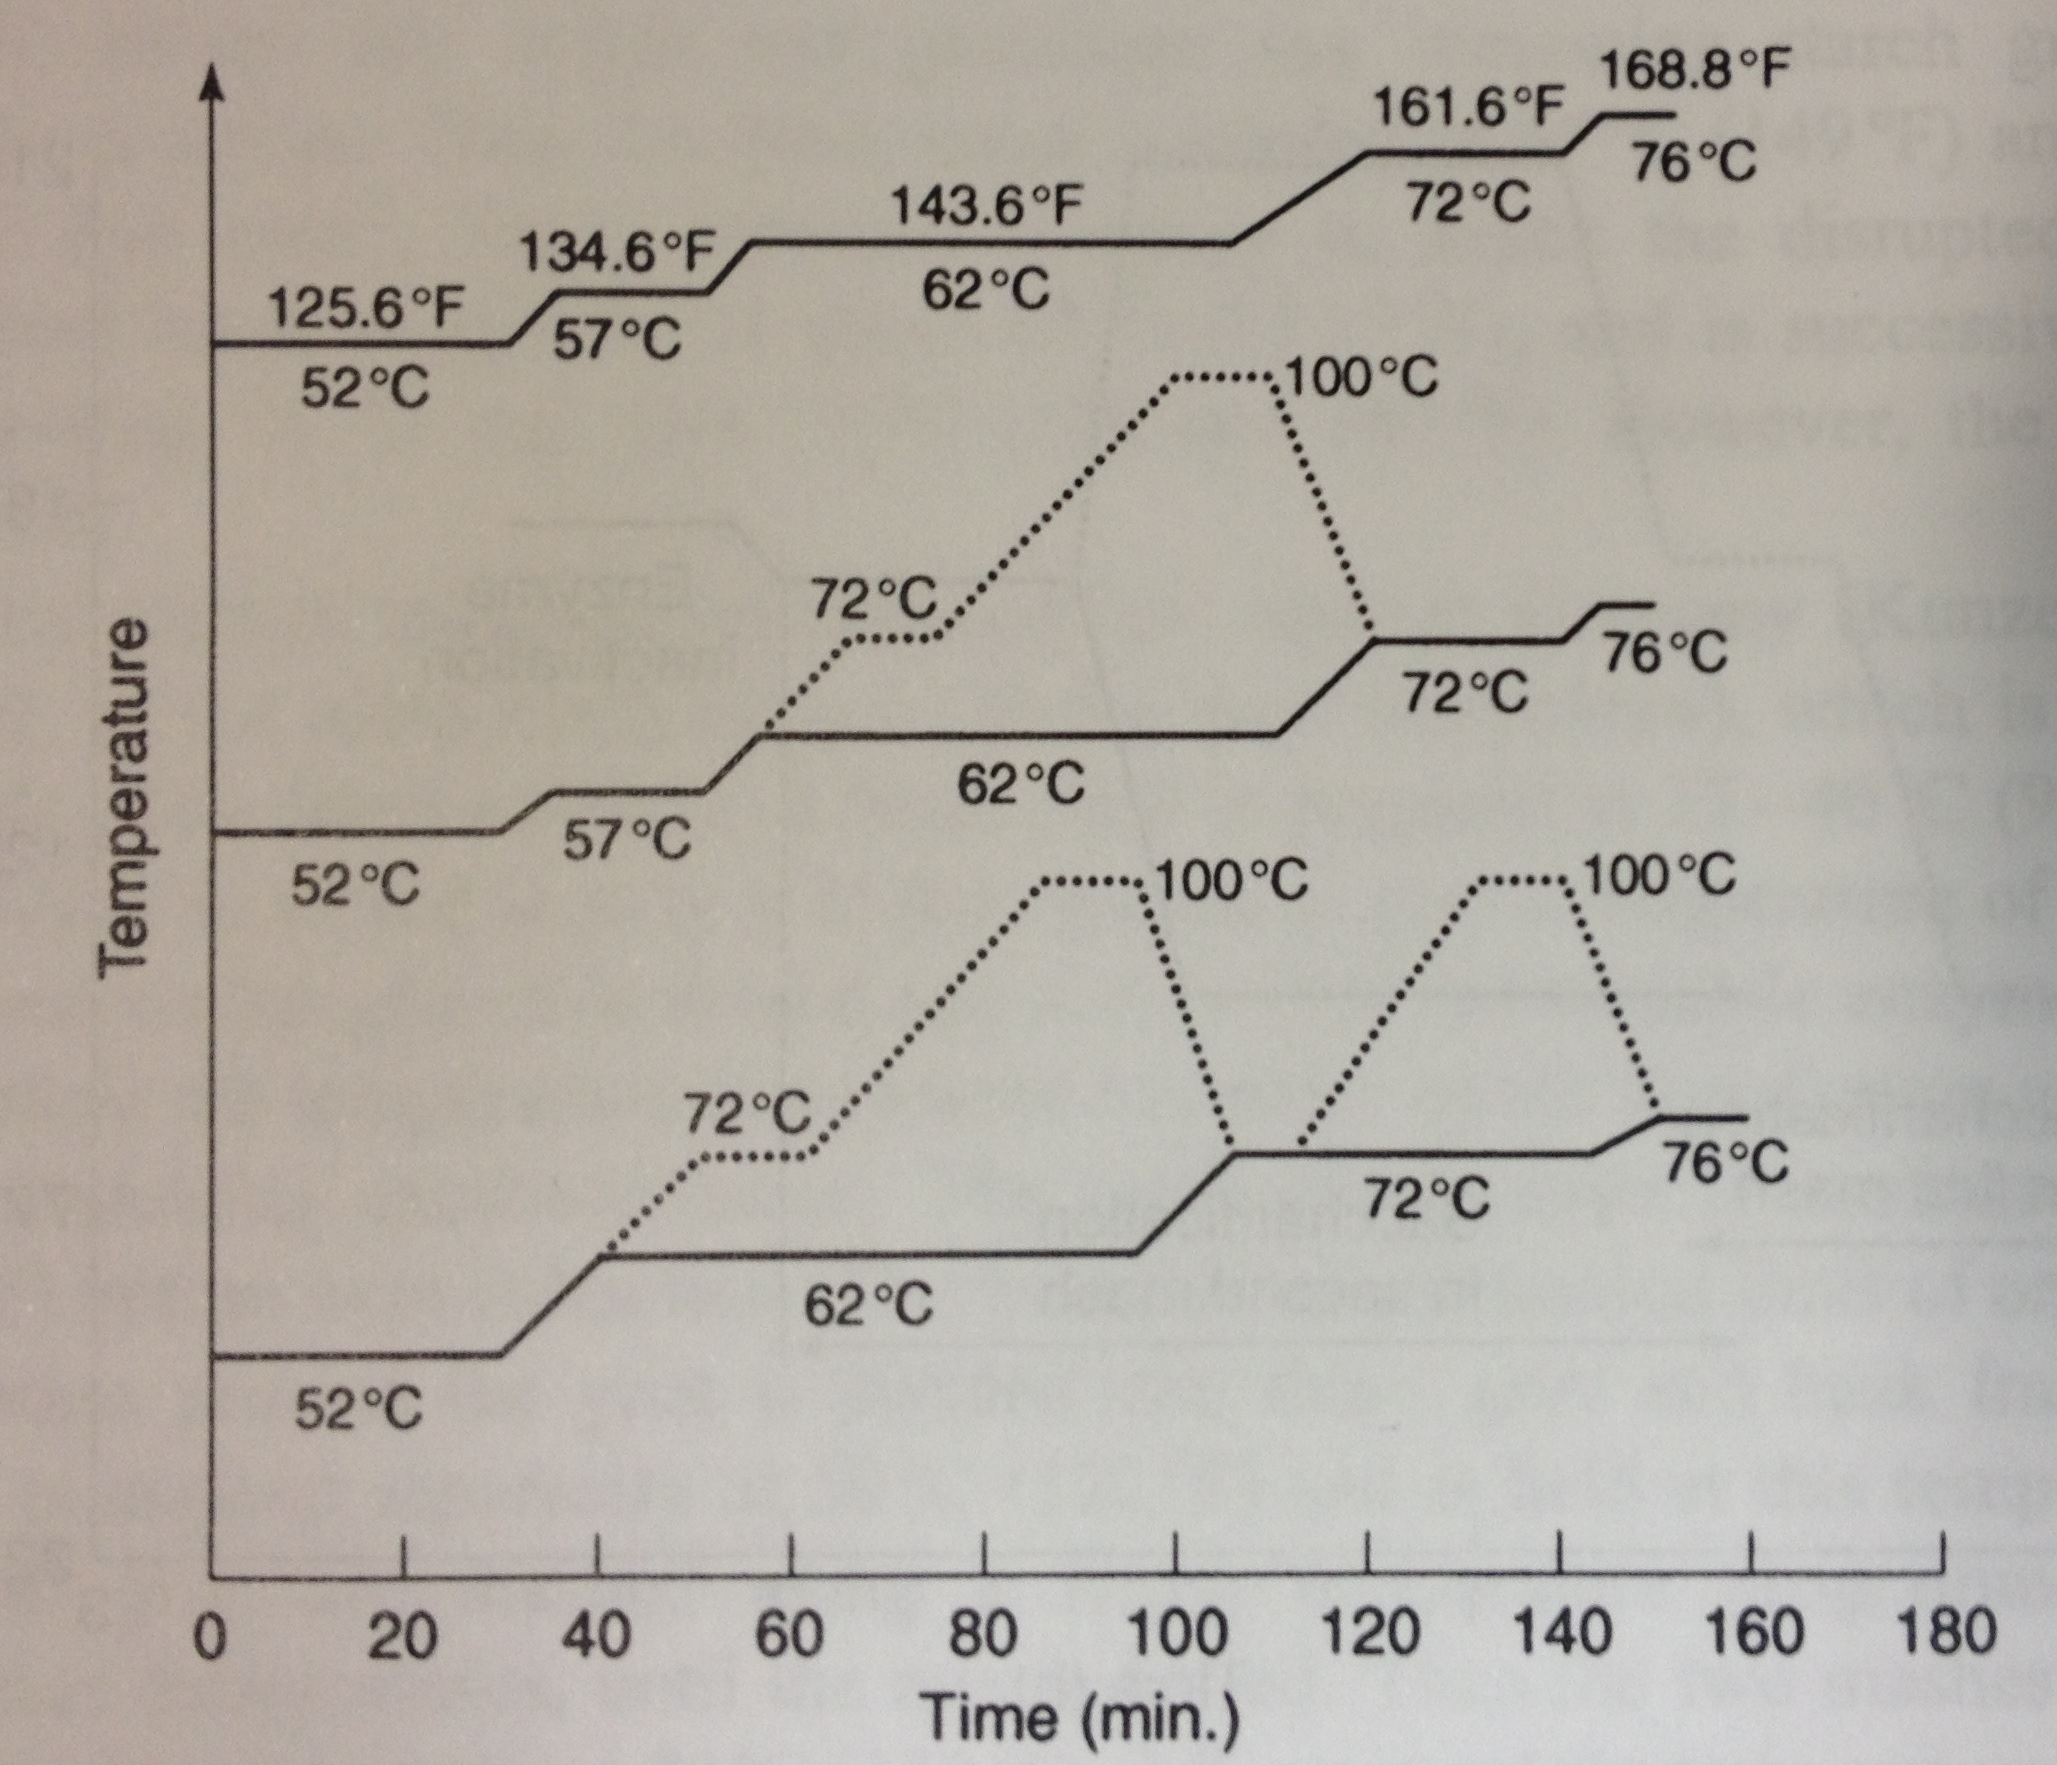
\includegraphics[scale=0.20]{./Resources/exRampas.jpg}
	\captionsetup{justification=centering}
	\caption[Programa de temperaturas t�pico de uma brassagem.]{Programa de temperaturas t�pico de uma brassagem. \\Fonte: BRIGGS (2011)
	}
	\label{exRampa}
\end{figure}

Ap�s a \textbf{filtragem} do extrato do mosto, este � transferido para um caldeir�o de \textbf{fervura}, processo no qual s�o adicionados os l�pulos e que leva cerca de uma hora, podendo se extender dependendo da receita \cite{briggs}, a exemplo das cervejas comerciais \textit{90 Minute IPA} e \textit{120 Minute IPA}, da cervejaria Dogfish Head, cujos tempos de fervura duram 90 minutos e 120 minutos, respectivamente \cite{1001,dogfish}. L�pulo � uma flor em formato de cone e � utilizado para conferir amargor e aroma � cerveja, al�m de ser um �timo conservante natural. Pode ser adicionado ao mosto em flores, \textit{pellets} (pastilhas prensadas) ou extrato. Quando adicionado no in�cio da fervura, contribui para o amargor da cerveja, por meio da isomeriza��o de �cidos alfa que ocorre em fun��o da alta temperatura. Em contrapartida, compostos arom�ticos vol�teis s�o perdidos neste processo e, por isso, tamb�m � adicionada uma quantidade de l�pulos ao final da fervura, para contribuir com o aroma \cite{palmer,briggs}.

Al�m de conferir amargor � cerveja, por meio da adi��o de l�pulos, a fervura tamb�m � respons�vel pela coagula��o de prote�nas indesej�veis, assepsia do l�quido, evapora��o e consequente redu��o do seu volume, mudan�as no sabor da cerveja e evapora��o de compostos vol�teis indesej�veis \cite{briggs}.

Na sequ�ncia da fervura, o mosto deve ser \textbf{resfriado} rapidamente at� 26\textdegree C para evitar oxida��o, contamina��o e cria��o de compostos org�nicos que introduzem sabores indesejados \cite{palmer}. O processo de resfriamento � realizado com o emprego de um trocador de calor, denominado \textit{chiller}. Tamb�m devem ser separadas e desprezadas as prote�nas coaguladas e os restos de l�pulos decorrentes da fervura. Este processo geralmente � denominado \textit{whirlpool}, em fun��o de sua natureza, na qual o mosto fervido � centrifugado e os compostos indesejados se acumulam no centro e no fundo da panela de fervura \cite{briggs}. O �ltimo passo � aerar ou at� mesmo oxigenar o mosto, para que as leveduras possam se reproduzir corretamente no in�cio da \textbf{fermenta��o} \cite{briggs}.

A levedura deve ser adicionada ao mosto resfriado e oxigenado o mais r�pido poss�vel para evitar contamina��es, e o recipiente de fermenta��o comumente � selado, evitando a entrada de ar \cite{briggs}. O processo de fermenta��o e os subsequentes processos de \textbf{matura��o} e \textbf{envase} n�o ser�o detalhados, pois sua automa��o n�o � parte do escopo deste trabalho e o tema destes t�picos, em conjunto com a fermenta��o, envolve quase que exclusivamente outras �reas do conhecimento n�o relacionadas � engenharia el�trica.


\section{Estrutura mec�nica}
O processo de brassagem, que consiste no cozimento dos maltes para extra��o dos a��cares ferment�veis e filtra��o do l�quido resultante, conhecido como mosto, � realizado em equipamentos espec�ficos para estas tarefas. Em fun��o das diferentes t�cnicas de brassagem e tecnologias desenvolvidas ao longo do tempo, diversos tipos e arranjos de equipamentos foram desenvolvidos \cite{briggs}.

Atualmente existe uma converg�ncia nos m�todos de fabrica��o de cervejas, motivada principalmente por quest�es financeiras, cujo objetivo do equipamento � maximizar a produ��o. Outros motivos para o desenvolvimento e aprimoramento de equipamentos s�o a necessidade de sempre produzir uma cerveja com as mesmas caracter�sticas, ou seja, padronizar a produ��o e, tamb�m, a preocupa��o crescente com redu��o do uso de energia e �gua e a redu��o da produ��o de efluentes \cite{briggs}. Ainda assim, equipamentos antigos continuam em uso, seja pela impossibilidade de reproduzir a cerveja em equipamentos mais modernos ou pelo custo elevado da atualiza��o das plantas de produ��o.

Na adi��o dos gr�os � panela de mostura, o processo de mistura destes � �gua � importante para que a brassagem seja eficiente, uma vez que os gr�os mal misturados podem formar aglutinados que impedem a extra��o dos a��cares. Para evitar este inconveniente, dispositivos mec�nicos foram desenvolvidos, conforme exposto na figura \ref{mashin}: em (a) a �gua e os gr�os s�o misturados em um fluxo constante, determinado pela velocidade de giro de uma rosca sem fim e; em (b) a �gua � adicionada aos maltes em um �ngulo tangente, de tal forma que um v�rtex a mistura aos gr�os.  A temperatura da �gua tamb�m deve ser controlada, para evitar que prote�nas sejam inativadas e seu volume inicial � predeterminado conforme a receita \cite{briggs}.

\begin{figure}[H]
	\centering
	\begin{subfigure}{.59\textwidth}
		\centering
		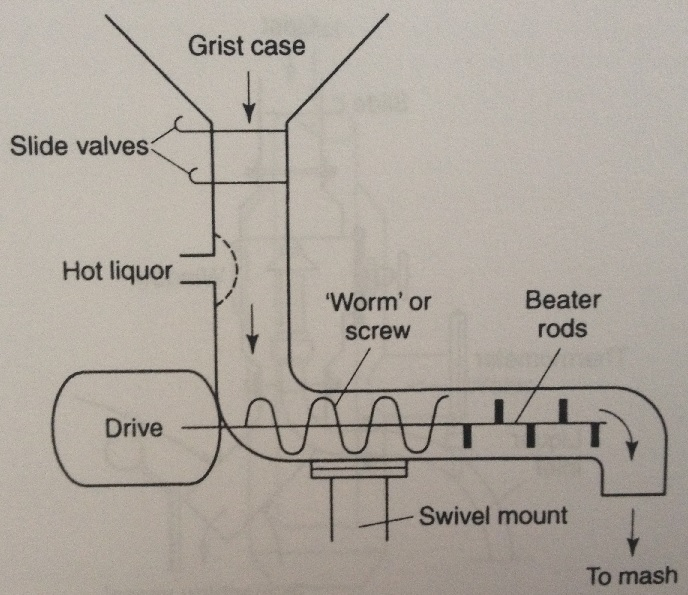
\includegraphics[height=5cm]{./Resources/mashin.jpg}
		\caption{Dispositivo com rosca sem fim}
		\label{mashin:1}
	\end{subfigure}
	\begin{subfigure}{.4\textwidth}
		\centering
		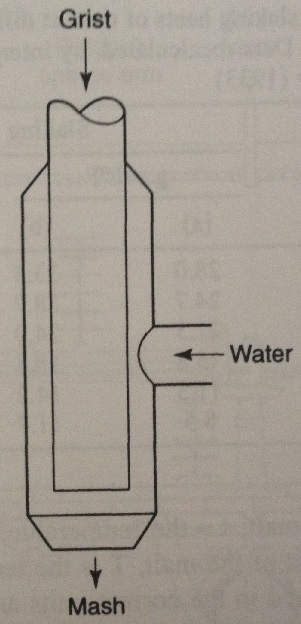
\includegraphics[height=5cm]{./Resources/mashin1.jpg}
		\caption{Dispositivo de mistura por v�rtex}
		\label{mashin:2}
	\end{subfigure}
	\captionsetup{justification=centering}
	\caption[Dispositivos de mistura de gr�os � brassagem.]{Dispositivos de mistura de gr�os � brassagem. \\Fonte: BRIGGS (2011)
	}
	\label{mashin}
\end{figure}

\subsection{Panela de mostura}

A panela de mostura, ou MT (\textit{mash tun}), � o dispositivo mais simples para a prepara��o do mosto, uma vez que nela ocorre a extra��o dos a��cares, a filtra��o do extrato do mosto e a lavagem dos gr�os \cite{briggs}. A figura \ref{mashTun} apresenta uma configura��o comum de MT, usada atualmente.

\begin{figure}[H]
	\centering
	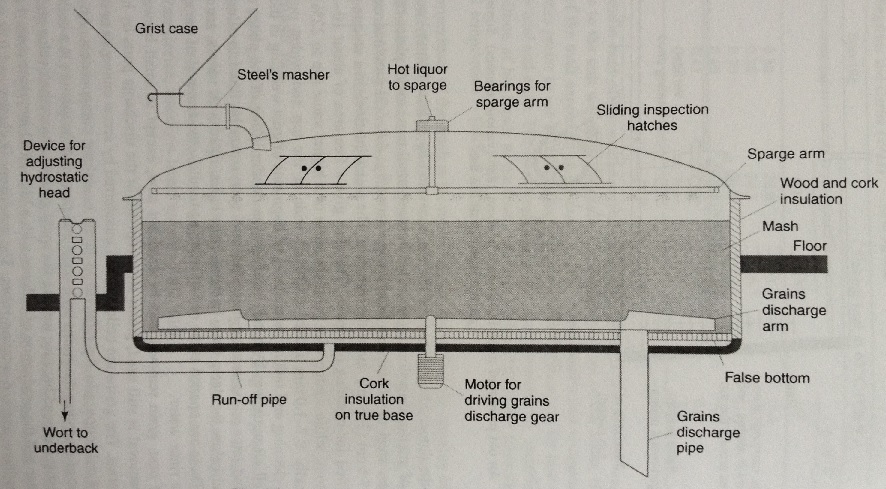
\includegraphics[scale=0.55]{./Resources/mt_modern.jpg}
	\captionsetup{justification=centering}
	\caption[Esquema de panela de brassagem industrial moderna.]{Esquema de panela de brassagem industrial moderna. \\Fonte: BRIGGS (2011)
	}
	\label{mashTun}
\end{figure}

As MTs possuem se��o transversal circular e atualmente s�o feitas de a�o inoxid�vel, revestidas com material isolante t�rmico. Embora originalmente fossem abertas, atualmente s�o cobertas para evitar perda de calor e espalhamento do vapor de �gua pelo ambiente da brassagem. O fundo da MT � coberto por um fundo falso, que fica a alguns cent�metros acima do fundo original e cuja fun��o � atuar como filtro, em conjunto com a cama de gr�os. Este fundo falso consiste de uma ou mais chapas de metal com rasgos da ordem de 0,7-1,0mm, que representam uma �rea livre para a drenagem de cerca de 12\% da �rea total, ou uma trama com fios de metal cuja �rea livre chega a 22\% \cite{briggs}.

O descarte dos gr�os � feito atrav�s de um tubo, com a ajuda de uma p� que varre o fundo da panela ou um jato de ar comprimido. M�todos de remo��o dos gr�os descontinuados s�o a remo��o manual (que ainda existe em pequenas instala��es) e o enx�gue dos gr�os com bombeamento para um tanque anexo -- este n�o mais usado em fun��o da necessidade de mais �gua e posterior tratamento desta, que resulta em custos adicionais, al�m da perda do valor comercial dos gr�os a serem descartados. Com rela��o � limpeza, as MTs s�o constru�das com suporte � limpeza CIP (limpeza no local), inclusive na regi�o entre o fundo da panela e o fundo falso \cite{briggs}.

A �gua da lavagem dos gr�os, ou \textit{sparging}, � borrifada por um cano ou mais canos suspensos acima da cama de gr�os, conforme ilustrado na figura \ref{mashTun}. Estes canos s�o conhecidos como bra�os de \textit{sparging} e geralmente giram no eixo em fun��o da for�a da �gua, o que s� � poss�vel devido aos furos no tubo serem feitos na vertical, especialmente para este prop�sito. Outro aspecto da constru��o dos bra�os de \textit{sparging} � que, � medida que se aproxima do centro da panela, os furos s�o feitos a uma dist�ncia menor entre si, possibilitando que a �gua seja igualmente distribu�da sobre a cama de gr�os \cite{briggs}. O extrato do mosto � coletado por tubos no fundo da panela.

No caso da brassagem feita pelo processo de decoc��o, brassagem dupla ou infus�o por temperatura controlada, diferentes recipientes de brassagem s�o utilizados. A figura \ref{mashMixer} � um exemplo de tina de mistura (n�o confundir com mostura, embora a panela seja utilizada no processo de mostura) usada para brassagem de temperatura controlada. Nestes casos, a moagem dos maltes � mais fina e estes s�o constantemente misturados por uma p� no fundo da panela. Mesmo dentre estes sistemas os equipamentos diferem entre si e, diferente da MT, nestes sistemas � preciso utilizar outro recipiente para separar o extrato dos gr�os. O separador pode ser uma tina de lavagem, conhecida tamb�m como LT (\textit{lauter tun}), ou pode ser um filtro de mosto. Embora a LT e o filtro de mosto sejam amplamente utilizados na ind�stria, n�o ser�o detalhados neste trabalho, j� que a abordagem pr�tica adotada n�o inclui seu uso.

\begin{figure}[H]
	\centering
	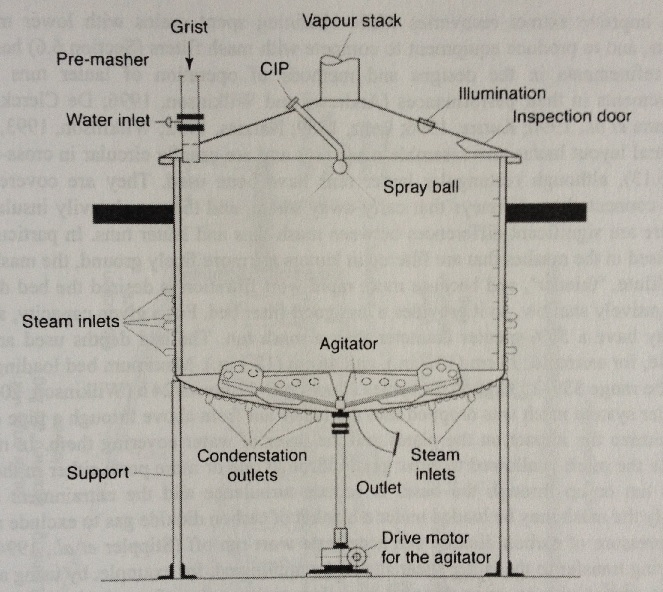
\includegraphics[scale=0.55]{./Resources/mt_mix.jpg}
	\captionsetup{justification=centering}
	\caption[Esquema de panela de mistura do mosto.]{Esquema de panela de mistura do mosto. \\Fonte: BRIGGS (2011)
	}
	\label{mashMixer}
\end{figure}

\subsection{Caldeir�o de fervura}

A fervura � o processo no qual o extrato do mosto � fervido com a adi��o de l�pulos em um caldeir�o de fervura. Em ingl�s o termo utilizado para este caldeir�o (\textit{copper}, que significa cobre) lembra o fato de que inicialmente era comum o emprego de tinas de cobre, dada a facilidade de moldagem que este metal permite, a alta condutividade t�rmica e a apar�ncia atrativa dos caldeir�es \cite{briggs}. Este tamb�m � usualmente referido como BK, ou \textit{brewing kettle} (caldeir�o de fervura). Por muito tempo o estudo do processo de fervura foi negligenciado por ser considerado simples, mas � medida que a quest�o da economia de energia veio � pauta, estudos oriundos desta necessidade mostraram que o processo � mais complicado do que foi inicialmente considerado \cite{briggs}.

Como existe uma lista de objetivos que devem ser cumpridos durante o processo de fervura, o projeto do equipamento � essencial para que estes sejam atingidos e, em um grau mais avan�ado, a maior economia de energia possa ser obtida. O primeiro objetivo -- que n�o est� necessariamente em ordem de import�ncia -- � a evapora��o de �gua e consequente concentra��o do mosto, com taxas de evapora��o inicialmente na faixa de 10\% do volume por hora e que foram reduzidas com o desenvolvimento tecnol�gico das grandes ind�strias, j� que o custo de evapora��o da �gua � caro em termos de demanda energ�tica. O segundo objetivo importante da fervura � esterilizar o mosto, ou pelo menos matar formas vegetativas de micr�bios -- ainda que esporos possam sobreviver ao processo. A terceira fun��o do processo � a evapora��o de compostos vol�teis indesejados, o que resultou em um desafio tecnol�gico para diminuir os tempos de fervura e quantidade de �gua evaporada sem que os compostos vol�teis deixassem de ser eliminados efetivamente \cite{briggs}.

Dentre as mudan�as que ocorrem no mosto durante a fervura, podem ser notadas cria��es, adi��es e transforma��es de subst�ncias qu�micas, como a dispers�o de resinas e �leos do l�pulo no mosto e a isomeriza��o de �cidos-\si{\alpha} (transforma��o dos �cidos-\si{\alpha} presentes no l�pulo em is�meros que conferem caracter�sticas de amargor � bebida), al�m da desnatura��o e forma��o de co�gulos de prote�nas -- processo que � favorecido por uma fervura rigorosa e prolongada -- que vir�o a formar o chamado \textit{trub}, resultado da decanta��o destas prote�nas.  Este processo de decanta��o pode ser acelerado por meio da adi��o de subst�ncias como gel de s�lica ou musgo irland�s, conhecido como \textit{irish moss} \cite{briggs}.

Historicamente o aquecimento dos BKs era feito de forma direta, com a queima de combust�veis s�lidos. Embora estes n�o sejam empregados atualmente, ainda existem BKs que s�o aquecidos diretamente, por meio da queima de �leos ou gases. Ainda assim, atualmente o maior elemento de aquecimento utilizado � o vapor d'�gua. Embora estes sistemas sejam mecanicamente mais complexos, o aquecimento a vapor reduz a quantidade de calor aplicada por unidade de �rea, o que evita a carameliza��o do mosto \cite{briggs}. Na figura \ref{boilcopper} s�o apresentadas tr�s configura��es de BKs, sendo (a) e (b) por meio de aplica��o direta de vapor � superf�cie do recipiente e (c) utilizando um aquecedor interno, tamb�m a vapor.

\begin{figure}[H]
	\centering
	\begin{subfigure}{.46\textwidth}
		\centering
		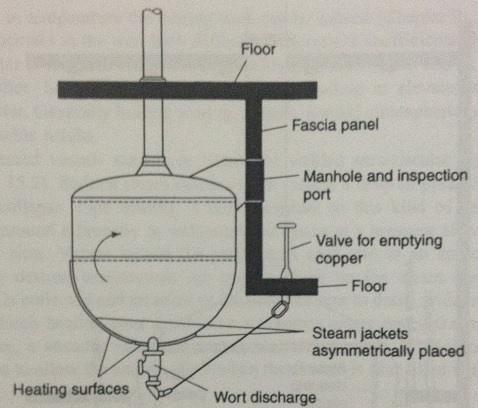
\includegraphics[height=5cm]{./Resources/boil_steam1.jpg}
		\caption{Caldeir�o com base arredondada e revestimentos de vapor assimetricamente dispostos}
		\label{boilcopper:1}
	\end{subfigure}
	\begin{subfigure}{.46\textwidth}
		\centering
		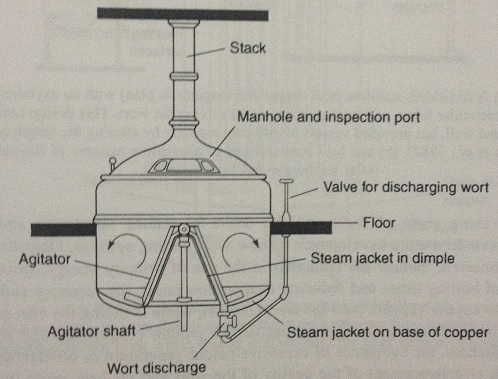
\includegraphics[height=5cm]{./Resources/boil_steam2.jpg}
		\caption{Caldeir�o de alta efici�ncia, com revestimentos de vapor na base e no cone central}
		\label{boilcopper:2}
	\end{subfigure}
	\begin{subfigure}{.65\textwidth}
		\centering
		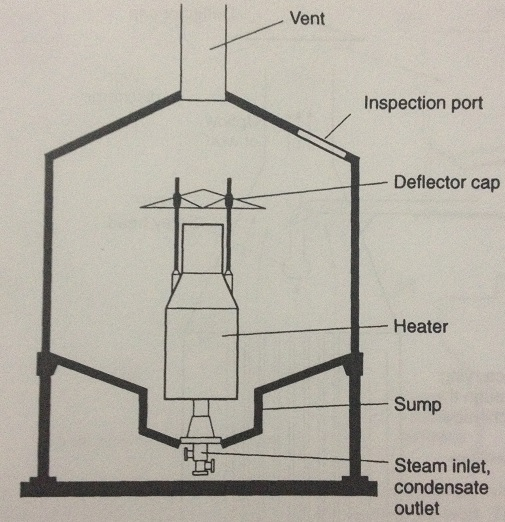
\includegraphics[height=5cm]{./Resources/boil_internal.jpg}
		\caption{Caldeir�o com aquecimento interno e mais profundo no centro, permitindo um aquecedor maior}
		\label{boilcopper:3}
	\end{subfigure}
	\captionsetup{justification=centering}
	\caption[Diferentes configura��es de caldeir�es de fervura.]{Diferentes configura��es de caldeir�es de fervura. \\Fonte: BRIGGS (2011)
	}
	\label{boilcopper}
\end{figure}

O projeto destes sistemas mec�nicos s�o feitos com o objetivo de evitar que o mosto seja caramelizado ou descaracterizado de alguma forma e de modo a economizar energia. Com isso surgiram em fun��o do tempo sistemas pressurizados e de aquecimento externo do l�quido, dentre outras configura��es diversas. Todos os sistemas modernos e eficientes de fervura s�o fechados e se aproveitam da pressuriza��o de algum modo para reduzir o custo energ�tico do processo de fervura, que se d� pela redu��o do tempo de fervura possibilitada pela eleva��o da temperatura do mosto. Contudo � preciso atentar-se ao fato de que temperaturas muito altas podem afetar negativamente a produ��o da cerveja e, portanto, valores t�picos de temperatura empregados pela ind�stria chegam a at� 104\si{\degree}C, com exce��es\footnotemark \cite{briggs}. A tabela \ref{tipos_fervura} apresenta alguns sistemas de fervura utilizados na ind�stria e suas caracter�sticas com rela��o a temperatura, tempo de fervura e evapora��o do mosto. Note-se que mesmo para um tipo espec�fico de fervura, diversas configura��es de equipamento podem ser adotadas.

\footnotetext{O sistema de alta temperatura / alta press�o (140\si{\degree}C) � pouco utilizado e testes pr�ticos mostram que os resultados em termos de qualidade da cerveja s�o question�veis \cite{briggs}}

\begin{center}
	\begin{table}[H]
		\captionsetup{justification=centering}
		\caption[Caracter�sticas de diferentes sistemas de fervura.]{Caracter�sticas de diferentes sistemas de fervura. \\Fonte: adaptado de BRIGGS(2011)}
		\label{tipos_fervura}
		\begin{tabular}{ | M{6cm}  M{3cm}  M{3cm}  M{3cm} |}
			\hline
			\textbf{Sistema de aquecimento} & \textbf{Temperatura (\si{\degree}C)} & \textbf{Tempo de fervura (min.)} & \textbf{Evapora��o (\%)} \\ \hline
			Panela de "alta performance" & 100 & 120-150 & 12-16 \\
			Aquecedores internos/externos, com contrapress�o & 102-103 & 60-80 & 8 \\
			Fervura de baixa press�o & 103-104 & 55-65 & 6-7 \\
			Fervura din�mica de baixa press�o & 103-104 & 45-50 & 4,5-5 \\
			Fervura de alta temperatura / alta press�o & 130-140 & 2,5-3 & 6-8 \\
			Aquecimento de pel�cula fina & 100 & 35-40 & 4-4,7\\ \hline
		\end{tabular}
	\end{table}
\end{center}

Embora o objetivo principal deste trabalho n�o seja a efici�ncia energ�tica do sistema, neste par�grafo s�o apresentadas algumas considera��es acerca do tema. Uma vez que o aquecimento de �gua une todas as partes do processo de produ��o de cerveja, n�o � realista acreditar que a economia de energia pode ser aplicada exclusivamente ao processo de fervura, que � o mais custoso em termos energ�ticos, portanto automa��o de controles, equipe bem capacitada, boa conserva��o do edif�cio, \textit{designs} eficientes, dentre outros fatores, s�o importantes para a economia de energia. No tocante � fervura em espec�fico, geralmente s�o utilizados sistemas que recuperam energia de vapor e/ou �gua quente para reuso nas diversas etapas do processo de produ��o de cerveja \cite{briggs}. Um exemplo � o sistema da figura \ref{eng_sav}, que utiliza energia do vapor de aquecimento utilizado na fervura para posterior aquecimento do mosto e pr�-aquecimento de outra fervura. Para que isto seja poss�vel, � essencial que a cervejaria realize consecutivas produ��es, uma vez que a energia � transferida para a produ��o seguinte.

\newpage

\begin{figure}[H]
	\centering
	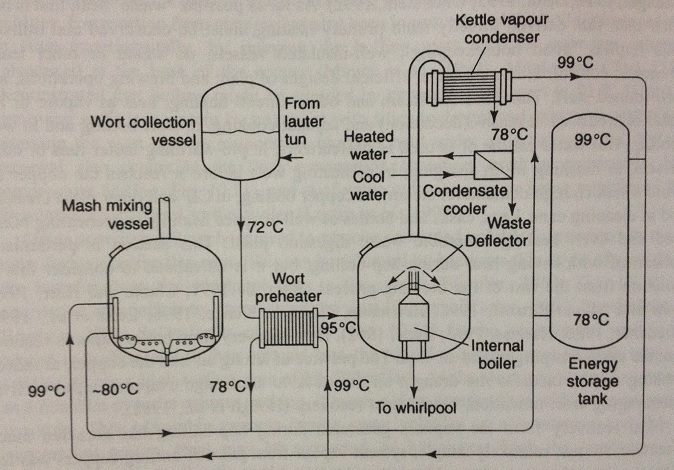
\includegraphics[scale=0.5]{./Resources/energy_saving.jpg}
	\captionsetup{justification=centering}
	\caption[Arranjo para recupera��o de energia.]{Arranjo no qual vapor do caldeir�o de fervura � condensado e calor � recuperado e armazenado como �gua quente em um tanque de gradiente de temperatura. \\Fonte: BRIGGS (2011)
	}
	\label{eng_sav}
\end{figure}

\subsection{Adi��o de l�pulos}

� comum realizar a adi��o de l�pulos manualmente em pequenas cervejarias, por�m deve-se observar que a adi��o de l�pulos pode ser uma tarefa perigosa, pois o mosto pode subitamente vazar. Tamb�m, em adi��es tardias de l�pulo, ocorre a entrada de ar no BK, o que faz com que sistemas pressurizados n�o possam ser utilizados sem as devidas considera��es e/ou modifica��es no equipamento \cite{briggs}.

A adi��o de l�pulos geralmente n�o � satisfat�ria quando s�o utilizadas flores, por isso pastilhas ou extratos s�o geralmente utilizados. Em grandes cervejarias a maior parte do desafio est� no fato de que os l�pulos devem ser armazenados em ambientes com temperatura controlada, que geralmente ficam longe do BK, al�m de serem armazenados em caixas ou tanques. Al�m do sistema autom�tico de transporte destes pacotes, em caso de BKs com pressuriza��o, � preciso utilizar sistemas de c�maras de compress�o para adicionar os l�pulos � panela \cite{briggs}.

\subsection{Clarifica��o e resfriamento do mosto}
Quando o processo de fervura � finalizado, o mosto dever� estar claro, ou seja, com apar�ncia brilhante. Ainda assim, � preciso remover o \textit{trub}\footnotemark \footnotetext{O \textit{trub} descrito neste cap�tulo � referente ao \textit{hot break}, ou processo de fervura. Neste trabalho n�o ser� abordado o \textit{trub} decorrente do \textit{cold break}, ou resfriamento do mosto, que come�a a ser formado em temperaturas pr�ximas a 70\si{\degree}C} e os restos de l�pulos utilizados no processo, j� que o \textit{trub} contribui com compostos sulfurosos e alco�is indesejados, al�m de tornar a cerveja turva -- o que pode ou n�o ser um problema \cite{byown}. Diversos equipamentos foram criados com este prop�sito, seja para mostos com adi��o de l�pulos em flores, que facilitam a extra��o dos compostos indesej�veis, quanto para mostos feitos com pastilhas e extratos de l�pulo. H� sistemas chamados \textit{hop back} empregados na filtragem de mostos com l�pulos em flor e que lembram MTs, nos quais o mosto � filtrado por um fundo falso, com elemento filtrador sendo a cama de l�pulos que decanta para o fundo da panela -- inclusive h� pequenas cervejarias que utilizam a MT para realizar este m�todo de clarifica��o \cite{briggs}.

Embora existam outros sistemas de clarifica��o, o empregado mais largamente na ind�stria atual � a t�cnica de \textit{whirlpool} (redemoinho, em tradu��o livre) na qual mosto quente � injetado tangencialmente em um recipiente cil�ndrico, a uma velocidade fixa, sendo a altura de inje��o do mosto vari�vel em fun��o de diferentes projetos. Sistemas de gravidade geralmente n�o s�o suficientes e bombas ou sistemas projetados para utilizar o efeito de termossif�o s�o utilizadas. As correntes de circula��o do mosto decorrentes desta inje��o tangencial fazem com que o material particulado fique concentrado no fundo e no centro do recipiente, possibilitando o escoamento controlado do l�quido e a consequente separa��o do \textit{trub} \cite{briggs}. Na figura \ref{whirlpool} s�o ilustrados sistemas de separa��o por decanta��o (a) e por \textit{whirlpool} (b).


\begin{figure}[H]
	\centering
	\begin{subfigure}{1.0\textwidth}
		\centering
		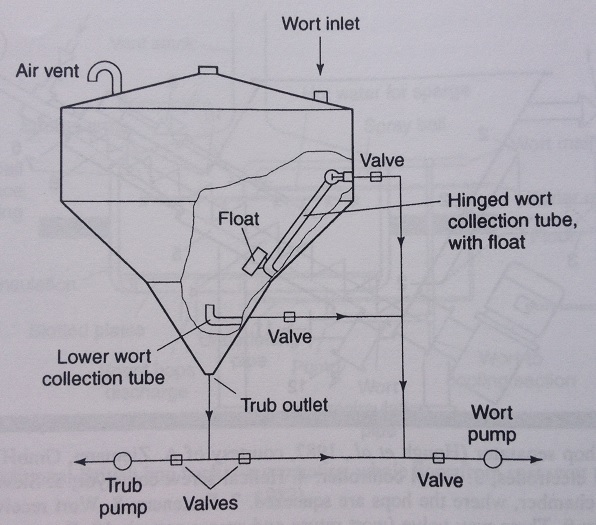
\includegraphics[height=5cm]{./Resources/trub_decanter.jpg}
		\caption{Sistema de serapa��o do \textit{trub} por decanta��o}
		\label{whirlpool:1}
	\end{subfigure}
	\begin{subfigure}{1.0\textwidth}
		\centering
		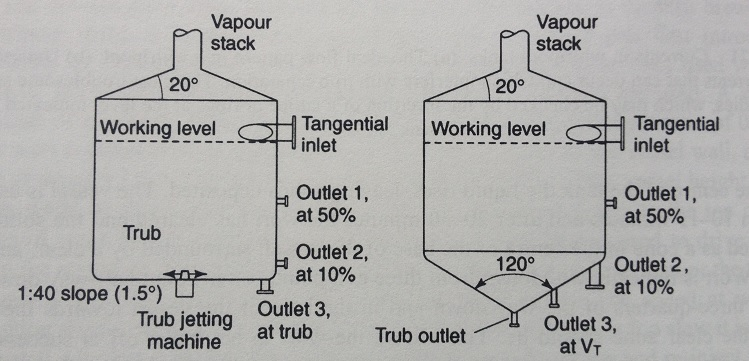
\includegraphics[height=5cm]{./Resources/trub_whirlpool.jpg}
		\caption{Sistemas de separa��o do \textit{trub} por \textit{whirlpool}, com fundo plano e arredondado}
		\label{whirlpool:2}
	\end{subfigure}
	\captionsetup{justification=centering}
	\caption[Sistemas de clarifica��o.]{Sistemas de clarifica��o. \\Fonte: BRIGGS (2011)
	}
	\label{whirlpool}
\end{figure}

Ap�s o processo de clarifica��o deve come�ar a fermenta��o e, para que as leveduras possam ser inoculadas no mosto, este deve ser resfriado at� a temperatura ideal de opera��o destes microorganismos, que est� t�picamente na faixa 15-22\si{\degree}C para leveduras do tipo \textit{ale} e 6-12\si{\degree}C para leveduras do tipo \textit{lager}. O resfriamento r�pido do mosto deve ocorrer, pois assim rea��es qu�micas decorretes da fervura s�o interrompidas e a chance de contamina��o do mosto � reduzida \cite{briggs}.

Para isto, um \textit{cooler} (resfriador ou trocador de calor) � utilizado. Dentre os modelos mais largamente empregados encontra-se o \textit{cooler} vertical, no qual o mosto passa por dentro de um arranjo de tubos finos, enquanto na parte externa destes �gua fria � circulada em contra-fluxo. Ainda assim, o modelo de \textit{cooler} mais popular � do trocador de calor de placas, devido ao seu tamanho compacto, versatilidade e efici�ncia. As placas possuem padr�es de desenho de tal forma que, quando s�o compactadas, elas formam canais pelos quais o mosto � passado em contra-fluxo a um agente resfriador (�gua fria, por exemplo). Estes trocadores de calor s�o projetados para que o escoamento seja turbulento e, consequentemente, a troca de calor seja mais eficiente. Quando um agente resfriador diferente da �gua � utilizado, a manuten��o do sistema deve ser refor�ada, j� que vazamentos implicam na contamina��o do mosto \cite{briggs}. A figura apresenta um esquema de \textit{cooler} de placas.

 \begin{figure}[H]
 	\centering
 	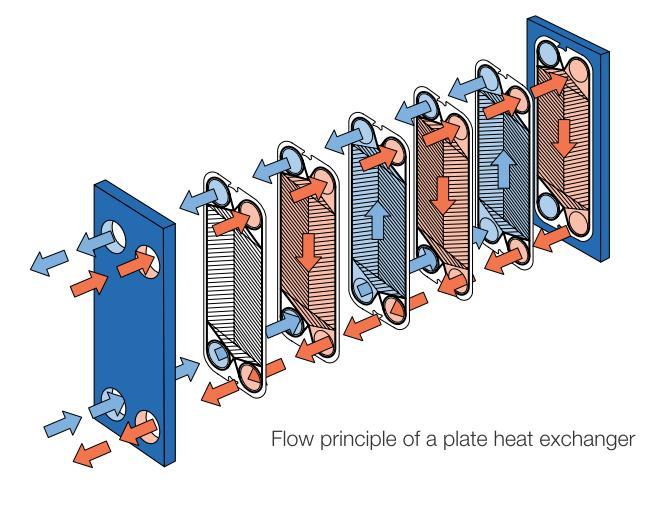
\includegraphics[scale=0.55]{./Resources/cooler.jpg}
 	\captionsetup{justification=centering}
 	\caption[Esquema de funcionamento do trocador de calor de placas.]{Esquema de funcionamento do trocador de calor de placas. \\Fonte: Site da Offshore Energy Today\protect\footnotemark
 	}
 	\label{usa-breweries}
 \end{figure}
 
 \footnotetext{Dispon�vel em \url{http://www.offshoreenergytoday.com/wp-content/uploads/2012/03/Alfa-Laval-to-Supply-Plate-Heat-Exchangers-for-Brazilian-Offshore-Plaforms.jpg}}

Por fim, antes de inocular a levedura, � importante que o mosto seja suficientemente aerado ou oxigenado. Sem isso, a levedura n�o ter� um ambiente adequado � sua reprodu��o e a atenua��o do mosto -- transforma��o de a��cares e oxig�nio em �lcool e g�s carb�nico -- n�o ser� completada. Diferen�as de solubilidade do mosto e dos tipos de levedura podem influenciar na quantidade de oxig�nio necess�ria para um bom andamento da fermenta��o, sendo que para obter os n�veis adequados, em escala industrial a oxigena��o geralmente � for�ada  \cite{briggs,palmer}. Na produ��o de cerveja artesanal, a aera��o geralmente � feita agitando o mosto resfriado ou com a ajuda de um sistema de aera��o de aqu�rio \cite{palmer}.


%\section{BeagleBone Black}
%BBB � uma placa de sistema embarcado desenvolvida para a comunidade de c�digo aberto (\textit{open-source}), iniciantes e quaisquer pessoas interessadas em um sistema equipado com um processador ARM Cortex-A8 32-bits de baixo custo, seja para teste de conceito ou mesmo uso pessoal/profissional. Embora o sistema tenha sido desenvolvido com um n�mero reduzido de funcionalidades, de modo a proporcionar uma boa experi�ncia de uso, esta placa n�o � uma plataforma completa de desenvolvimento nem � voltada para o desenvolvimento de um produto espec�fico, mas sim para a experimenta��o e aprendizado nas �reas de \textit{software} e \textit{hardware} \cite{bbb_srm}. A figura \ref{bbb} apresenta a placa e seus principais componentes, em conjunto com a tabela \ref{bbb_specs}, onde est�o contidas as especifica��es gerais de hardware e a figura \ref{bbb-bdg}, na qual est� contido um diagrama de blocos do sistema, de alto n�vel de abstra��o. O diagrama esquem�tico do sistema pode ser obtido no Anexo \ref{Anexo1}.

� imprescind�vel atentar para o fato de que a BBB possui diversas revis�es de \textit{hardware}, sendo que a vers�o utilizada neste trabalho � a \textbf{revis�o C}.

A combina��o do processador ARM Cortex-A8 com o projeto de \textit{hardware} da placa possibilita o uso de um sistema operacional embarcado -- geralmente uma distribui��o Linux -- que fornece facilidades de programa��o, a exemplo de uma IDE acessada pelo navegador da internet chamada Cloud9 em combina��o com uma biblioteca de acesso ao hardware em \textit{server-side} Javascript (Node.js), possibilitando a prototipagem r�pida de solu��es embarcadas de produtos voltados ao mundo real. � medida que o desenvolvedor do sistema se torna mais experiente, � poss�vel desenvolver solu��es mais complicadas em diversas linguagens de programa��o, utilizando-se para isto do sistema operacional Linux embarcado na placa. \cite{bbb_nannan}. Al�m disso, projetos como o do carro de controle remoto via web, desenvolvido por \cite{bbb_nannan} com o intuito de confirmar as capacidades de placa e seu potencial uso no ensino de sistemas embarcados, refor�am a escolha da BBB como plataforma para este projeto.  

\begin{figure}[H]
	\centering
	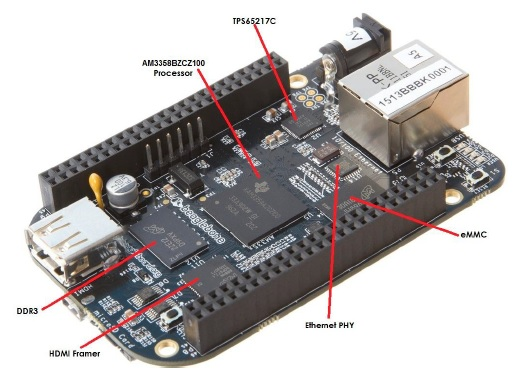
\includegraphics[scale=0.55]{./Resources/bbb-components.jpg}
	\captionsetup{justification=centering}
	\caption[BeagleBone Black e principais componentes]{BeagleBone Black e principais componentes. \\Fonte: COLEY (2014)
	}
	\label{bbb}
\end{figure}

\begin{itemize}
	\item \textbf{Sitara AM3358BZCZ100} - SoC (\textit{system on chip})
	\item \textbf{Micron 512MB DDR3L ou Kingston 512MB DDR3} - mem�ria RAM
	\item \textbf{TPS65217C PMIC} - controlador de alimenta��o dos diferentes componentes do sistema
	\item \textbf{SMSC Ethernet PHY} - interface f�sica � rede Ethernet
	\item \textbf{Micron eMMC} - mem�ria n�o vol�til MMC de 4GB
	\item \textbf{HDMI Framer} - controlador para uso com display HDMI ou DVI-D
\end{itemize}

\begin{center}
	\begin{table}[H]
		\captionsetup{justification=centering}
		\caption[Especifica��es Gerais da BeagleBone Black]{Especifica��es Gerais da BeagleBone Black. \\Fonte: adaptado de COLEY(2014)}
		\label{bbb_specs}
		\begin{tabular}{ | M{3cm} | M{12cm} |}
			\hline
			& \multicolumn{1}{|c|}{\textbf{Especifica��o}} \\ \hline
			Processador & Sitara AM3358BZCZ100, 1GHz, 2000 MIPS\\ \hline
			Motor Gr�fico & SGX530 3D, 20M pol�gonos/s \\ \hline
			Mem�ria SDRAM & 512MB DDR3L 800MHz \\ \hline
			Mem�ria Flash & 4GB, 8bit MMC embarcada \\ \hline
			CI Gerenciador de Alimenta��o & TPS65217C + regulador adicional (linear) \\ \hline
			Suporte a \textit{debug} & Interface serial, Conector CTI JTAG opcional de 20 pinos \\ \hline
			Fonte de Alimenta��o & mini USB, conector DC ou 5VDC na barra de pinos\\ \hline
			PCB & 8,64cm x 5,33cm (3,4" x 2,1") - 6 \textit{layers}\\ \hline
			Leds Indicadores & 1 para alimenta��o; 2 para Ethernet; 4 acess�veis ao usu�rio \\ \hline
			USB 2.0 \textit{Client} & Acesso � USB0 via miniUSB \\ \hline
			USB 2.0 \textit{Host} & Acesso � USB1, soquete tipo A, 500mA LS/FS/HS \\ \hline
			Serial & Acesso � UART0 via \textit{header} de 6 pinos, TTL 3.3V \\ \hline
			Ethernet & 10/100 RJ45 \\ \hline
			SD/MMC & Conector microSD, 3,3V \\ \hline
			Chaves & Bot�es push de reset, boot e alimenta��o \\ \hline
			Sa�da de v�deo & 16b HDMI, 1280x1024 (MAX), 1024x768, 1280x720, 1440x900, 1920x1080@24Hz \\ \hline
			Audio & Via interface HDMI, est�reo \\ \hline
			Conectores de expans�o & Alimenta��o 5V, 3,3V e VDD\_ADC(1,8V) \newline 3,3V para todos os sinais de E/S \newline McASP0, SPI, I2C, at� 69 pinos de GPIO, LCD, GPMC, MMC1, MMC2, 7 entradas para conversor A/D (1,8V MAX), 4 \textit{timers}, 4 UART, CAN, PWM via \textit{hardware}, interrup��o XDMA\\ \hline
			Peso & 39,68g (1,4oz) \\ \hline
			Consumo@5VDC & Ocioso - 280mA \newline Carregando p�gina web - 430mA \newline \*O consumo varia conforme o desempenho \\
			\hline
		\end{tabular}
	\end{table}
\end{center}

\begin{figure}[H]
	\centering
	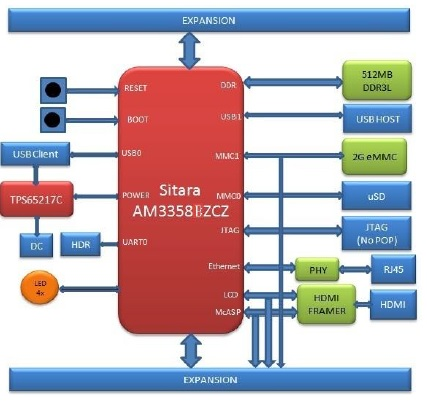
\includegraphics[scale=0.80]{./Resources/bbb-blockDG.jpg}
	\captionsetup{justification=centering}
	\caption[Diagrama de blocos de alto n�vel da BeagleBone Black]{Diagrama de blocos de alto n�vel da BeagleBone Black. \\Fonte: COLEY (2014)
	}
	\label{bbb-bdg}
\end{figure}

Cada pino de GPIO digital da BBB possui at� 7 modos diferentes de opera��o, que s�o configurados utilizando uma ferramenta do Linux chamada \textit{Device Tree}. A figura \ref{bbb_pins_def} apresenta a configura��o padr�o dos pinos, ou seja, quando � usada a distribui��o Angstrom do Linux, pr�-compilada e que � fornecida com a placa. Com rela��o aos pinos de GPIO, � importante notar que sua l�gica opera com n�veis de tens�o de 0V e 3,3V para os n�veis baixo e alto, respectivamente e portanto aplicar uma tens�o negativa ou superior a 3,3V pode danificar permanentemente a placa \cite{lumme}.

\begin{figure}[H]
	\centering
	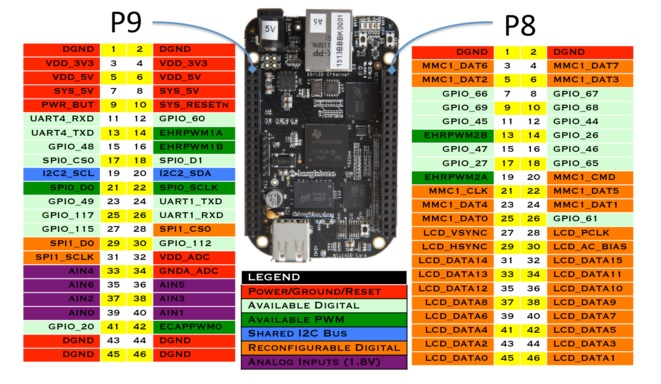
\includegraphics[scale=0.80]{./Resources/bbb-pins-def.jpg}
	\captionsetup{justification=centering}
	\caption[Configura��o padr�o dos pinos da BeagleBone Black]{Configura��o padr�o dos pinos da BeagleBone Black. \\Fonte: Site oficial da Funda��o BeagleBoard.org\protect\footnotemark
	}
	\label{bbb_pins_def}
\end{figure}

\footnotetext{Dispon�vel em \url{http://beagleboard.org/Support/bone101}}

\subsection{\textit{Programmable Real-time Unit -- PRU-ICSS}}

A PRU-ICSS -- \textit{Programmable Real-Time Unit Subsystem and Industrial Communications Subsystem} (Unidade Program�vel de Tempo-Real e Subsistema de Comunica��o Industrial, em tradu��o livre) � um subsistema do processador AM3358 que equipa a BBB, que � fabricado pela \textit{Texas Instruments} mas n�o tem suporte oficial da mesma \cite{bbb_srm}. Esta unidade consiste de dois n�cleos RISC de 32 bits, uma mem�ria compartilhada de 12kB, uma mem�ria de dados e uma mem�ria de programa para cada n�cleo, ambas com 8kB de capacidade e perif�ricos internos -- al�m da possibilidade de acessar todos os eventos, pinos e recursos do SoC AM3358 por meio de uma interface OCP, que confere a este subsistema grande flexibilidade. Cada n�cleo da PRU pode operar independentemente ou de maneira sincronizada, dependendo de como o \textit{firmware} para eles � escrito \cite{soc_manual}. Na figura � ilustrado o diagrama de blocos deste sistema.

\begin{figure}[H]
	\centering
	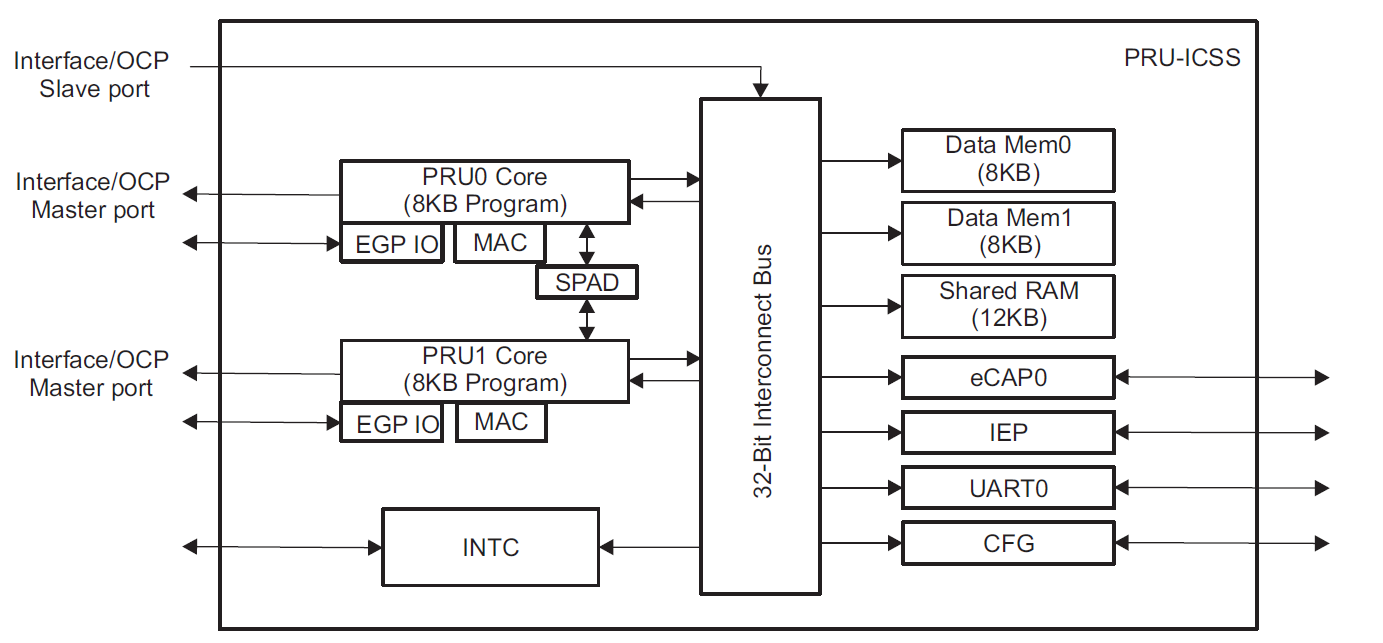
\includegraphics[scale=0.40]{./Resources/pru-blockDG.png}
	\captionsetup{justification=centering}
	\caption[Diagrama de blocos do subsistema PRU-ICSS]{Diagrama de blocos do subsistema PRU-ICSS. \\Fonte: TEXAS INSTRUMENTS (2015)
	}
	\label{pru-bdg}
\end{figure}

Os n�cleos da PRU foram otimizados para realizar tarefas com requisitos severos de tempo-real e, portanto, tem um \textit{clock} de 200MHz e um sistema de instru��es RISC no qual todas elas s�o executadas em um ciclo de \textit{clock}, propositalmente sem suporte a \textit{pipelining}. Cada n�cleo tem 31 registradores, cuja utiliza��o vai de prop�sito geral a indexa��o e controle de GPIO, acess�veis a n�vel de bit, byte, \textit{halfword} (16 bits), \textit{word} (32 bits) ou por ponteiro \cite{soc_manual}. Uma vez que cada instru��o pode ser executada em 5ns e o acesso a GPIO � feito por meio de uma �nica instru��o de acesso a registradores, isto significa que � poss�vel obter uma resolu��o de chaveamento determin�stica de no m�ximo 5ns, com dados obtidos na pr�tica, por \cite{bbb_pulsegen}, de \textit{jitter} RMS de 290ps e estabilidade de frequ�ncia na ordem de 10 ppm .

Uma vez que as diversas funcionalidades do m�dulo PRU s�o acessadas por meio de mapeamento da mem�ria de dados, � preciso saber a faixa de endere�o destas. Aqui deve ser feita a distin��o entre acesso � mem�ria local da PRU, que compreende os endere�os de 0x0000\_0000 a 0x0007\_FFFF, e o acesso � mem�ria global, cujos endere�os come�am em 0x0008\_0000. Tamb�m � importante notar que as mem�rias internas dos m�dulos podem ser acessados com o endere�o global de mem�ria, mas isso reduz significativamente o tempo de acesso, j� que o sinal � roteado para fora da PRU antes de ser recebido \cite{soc_manual}. Na tabela \ref{pru_localmem} � apresentado o mapa de mem�ria local e na tabela \ref{pru_globalmem} � apresentado o mapa de mem�ria global. Tamb�m h� uma tabela de constantes gravada em hardware, com valores de uso recorrente, para economizar instru��es de programa��o e registradores, nos quais estes endere�os precisariam ser carregados se n�o estivessem dispon�veis em hardware \cite{soc_manual}.

Embora cada PRU suporte 30 canais de entrada e 32 canais de sa�da no modo direto \cite{soc_manual}, a BBB roteia somente 25 pinos do SoC ao conector de expans�o. Destes, 10 pinos s�o exclusivos da PRU0 (8 sa�das ou 9 entradas) e 15 pinos para a PRU1 (13 sa�das ou 14 entradas). Eventualmente, alguns pinos pr�-configurados para outras fun��es devem ser reconfigurados antes que possam ser utilizados \cite{bbb_srm}. Os pinos da BBB acess�veis pela PRU podem ser obtidos na figura \ref{bbb_pins_pru}.

\begin{figure}[H]
	\centering
	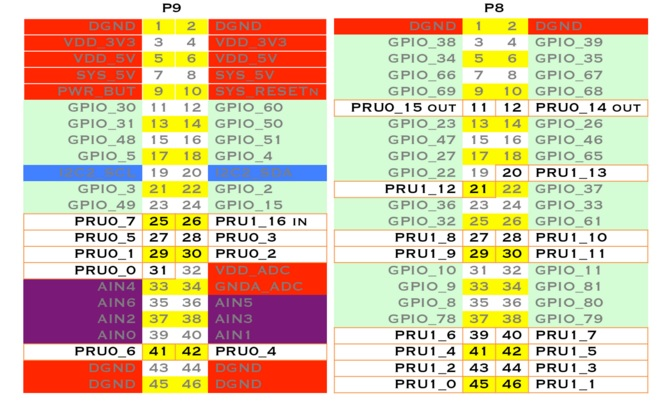
\includegraphics[scale=0.80]{./Resources/bbb-pins-pru.jpg}
	\captionsetup{justification=centering}
	\caption[Pinos da BeagleBone Black acess�veis pela PRU-ICSS]{Pinos da BeagleBone Black acess�veis pela PRU-ICSS. \\Fonte: Site oficial da Funda��o BeagleBoard.org\protect\footnotemark
	}
	\label{bbb_pins_pru}
\end{figure}

\footnotetext{Dispon�vel em \url{http://beagleboard.org/Support/bone101}}

\begin{center}
	\begin{table}[H]
		\captionsetup{justification=centering}
		\caption[Mapa de Mem�ria Local da PRU]{Mapa de Mem�ria Local da PRU. \\Fonte: adaptado de TEXAS INSTRUMENTS(2014)}
		\label{pru_localmem}
		\begin{tabular}{ | M{5cm} | M{5cm} | M{5cm} |}
			\hline
			\textbf{Endere�o Inicial} & \textbf{PRU0} & \textbf{PRU1} \\ \hline
			0x0000\_0000 & Mem. dados da PRU0 & Mem. dados da PRU1\\ \hline
			0x0000\_2000 & Mem. dados da PRU1 & Mem. dados da PRU0\\ \hline
			0x0001\_0000 & Mem. dados compartilhada & Mem. dados compartilhada \\ \hline
			0x0002\_0000 & INTC & INTC \\ \hline
			0x0002\_2000 & Controle da PRU0 & Controle da PRU0 \\ \hline
			0x0002\_2400 & Reservado & Reservado \\ \hline
			0x0002\_4000 & Controle da PRU1 & Controle da PRU1 \\ \hline
			0x0002\_4400 & Reservado & Reservado \\ \hline
			0x0002\_6000 & CFG & CFG \\ \hline
			0x0002\_8000 & UART0 & UART0 \\ \hline
			0x0002\_A000 & Reservado & Reservado \\ \hline
			0x0002\_C000 & Reservado & Reservado \\ \hline
			0x0002\_E000 & IEP & IEP \\ \hline
			0x0003\_0000 & eCAP0 & eCAP0 \\ \hline
			0x0003\_2000 & Reservado & Reservado \\ \hline
			0x0003\_2400 & Reservado & Reservado  \\ \hline
			0x0003\_4000 & Reservado & Reservado  \\ \hline
			0x0003\_8000 & Reservado & Reservado  \\ \hline
			0x0004\_0000 & Reservado & Reservado  \\ \hline
			0x0008\_0000 & System OCP\_HP0 & System OCP\_HP1 \\ \hline
		\end{tabular}
	\end{table}
\end{center}

As interfaces de interrup��o e de GPIO est�o contidas nos registradores R30 e R31: o registrador R31 � utilizado tanto para interface dos pinos configurados como entrada quanto para leitura e/ou gera��o de eventos de interrup��o, enquanto o registrador R30
retorna status ou muda o valor dos pinos configurados como sa�da, para leitura e escrita, respectivamente. Embora a entrada possa ser configurada nos modos de captura paralela de 16 bits e trem de pulsos de 28 bits, estes modos de opera��o n�o ser�o detalhados, j� que seu uso n�o est� contido no escopo deste projeto. O mesmo � v�lido para a sa�da, que al�m do modo direto, pode ser configurada para transmitir um trem de pulsos \cite{soc_manual}.

Outra caracter�stica da PRU � a exist�ncia de um IEP - \textit{Industrial Ethernet Peripheral} (Perif�rico Ethernet Industrial, em tradu��o livre), composto de um \textit{timer} para Ethernet industrial com 8 eventos de compara��o e uma porta digital de E/S. O \textit{timer} Ethernet industrial � simplesmente um temporizador de 32 bits e, portanto, pode ser utilizado para uso geral. � um contador positivo, cujo valor dos incrementos pode ser programado na faixa de 1-16, com compensador de uso opcional. Os 8 registradores comparadores permitem a cria��o de eventos cada vez que o valor do comparador corresponde ao do temporizador \cite{soc_manual}.

\begin{center}
	\begin{table}[H]
		\captionsetup{justification=centering}
		\caption[Mapa de Mem�ria Global da PRU]{Mapa de Mem�ria Global da PRU. \\Fonte: adaptado de TEXAS INSTRUMENTS(2014)}
		\label{pru_globalmem}
		\begin{tabular}{ | M{5cm} | M{10cm} |}
			\hline
			\textbf{Endere�o de Offset} & PRU-ICSS \\ \hline
			0x0000\_0000 & Mem. dados da PRU0 \\ \hline
			0x0000\_2000 & Mem. dados da PRU1 \\ \hline
			0x0001\_0000 & Mem. dados compartilhada \\ \hline
			0x0002\_0000 & INTC \\ \hline
			0x0002\_2000 & Controle da PRU0 \\ \hline
			0x0002\_2400 & Debug da PRU0 \\ \hline
			0x0002\_4000 & Controle da PRU1 \\ \hline
			0x0002\_4400 & Debug da PRU1 \\ \hline
			0x0002\_6000 & CFG \\ \hline
			0x0002\_8000 & UART0 \\ \hline
			0x0002\_A000 & Reservado \\ \hline
			0x0002\_C000 & Reservado \\ \hline
			0x0002\_E000 & IEP \\ \hline
			0x0003\_0000 & eCAP0 \\ \hline
			0x0003\_2000 & Reservado \\ \hline
			0x0003\_2400 & Reservado  \\ \hline
			0x0003\_4000 & IRAM da PRU0  \\ \hline
			0x0003\_8000 & IRAM da PRU1  \\ \hline
			0x0004\_0000 & Reservado  \\ \hline
		\end{tabular}
	\end{table}
\end{center}

No que diz respeito ao desenvolvimento de \textit{firmware} para a PRU, h� um conjunto de instru��es RISC em assembly, suportado por um conjunto de ferramentas que ajudam a gerar o arquivo bin�rio a ser carregado na mem�ria de programa. Alguns exemplos s�o o \textit{assembler}, \textit{archiver} e o \textit{linker} \cite{pru_assembly_tools}. Outra ferramenta de desenvolvimento proporcionada pela Texas Instruments � um compilador C/C++, que facilita a programa��o em n�veis de abstra��o elevados \cite{pru_compiler}. A figura \ref{pru_firmdev} apresenta um diagrama de blocos que ilustra os passos a serem executados desde compilar o c�digo C/C++ at� carregar o arquivo execut�vel na mem�ria de programa da PRU.

\begin{figure}[H]
	\centering
	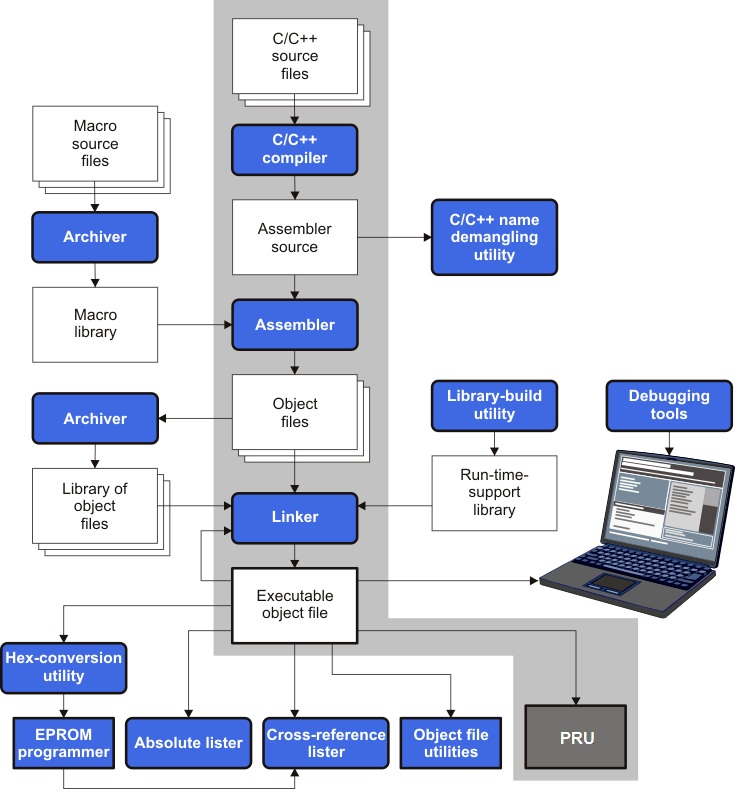
\includegraphics[scale=0.80]{./Resources/pru-software-dev.png}
	\captionsetup{justification=centering}
	\caption[Fluxo de desenvolvimento de software da PRU]{Fluxo de desenvolvimento de software da PRU. \\Fonte: TEXAS INSTRUMENTS
	}
	\label{pru_firmdev}
\end{figure}

\subsection{\textit{Device Tree}}

A \textit{Device Tree} ou DT � basicamente uma estrutura de dados utilizada para descrever \textit{hardware}, cujo objetivo � possibilitar que as caracter�sticas de \textit{hardware} de um sistema espec�fico sejam passadas para o SO durante o \textit{boot}, ao inv�s de estas informa��es ficarem gravadas no SO \cite{devicetree}, o que possibilita que um \textit{driver} do Kernel seja usado em configura��es diferentes de \textit{hardware} sem a necessidade de modifica��es em seu c�digo-fonte. Com rela��o aos sistemas equipados com processadores ARM, a necessidade de uso da DT surgiu devido ao grande n�mero de novas placas, que tornou muito dif�cil manter uma vers�o do Kernel para cada sistema. Seu objetivo n�o � modificar o sistema em tempo de execu��o, por�m no caso da BBB, foi criada uma solu��o chamada \textit{Device Tree Overlay} (ou sobreposi��o) para executar esta fun��o, facilitando a configura��o de GPIO, dentre outras fun��es, e uso da DT pelo usu�rio final \cite{bbb_devicetree}, fatores que s�o do interesse de aprendizes da �rea.

Uma DT � uma estrutura em �rvore, composta de n�s e propriedades. Uma abordagem para entender o seu funcionamento � por meio de um exemplo de sobreposi��o espec�fico para a BBB. Abaixo � apresentado um exemplo de sobreposi��o de DT espec�fico da BBB que apresenta os principais conceitos para o uso desta ferramenta:

\newpage

\lstset{language=dtc}
\begin{lstlisting}[frame=single, basicstyle=\linespread{0.85}\ttfamily]

/*
* Copyright (C) 2013 CircuitCo
*
* Virtual cape for UART1 on connector pins P9.24 P9.26
*
* This program is free software; you can redistribute it and/or modify
* it under the terms of the GNU General Public License version 2 as
* published by the Free Software Foundation.
*/
/dts-v1/;
/plugin/;

/ {
	compatible = "ti,beaglebone", "ti,beaglebone-black";

	/* identification */
	part-number = "BB-UART1";
	version = "00A0";
	
	/* state the resources this cape uses */
	exclusive-use =
		/* the pin header uses */
		"P9.24",        /* uart1_txd */
		"P9.26",        /* uart1_rxd */
		/* the hardware ip uses */
		"uart1";
	
	fragment@0 {
		target = <&am33xx_pinmux>;
		__overlay__ {
			bb_uart1_pins: pinmux_bb_uart1_pins {
				pinctrl-single,pins = <
		/* P9.24 uart1_txd.uart1_txd MODE0 OUTPUT (TX) */
					0x184 0x20
		/* P9.26 uart1_rxd.uart1_rxd MODE0 INPUT (RX) */ 
					0x180 0x20
				>;
			};
		};
	};
	
	fragment@1 {
		target = <&uart2>;	/* really uart1 */
		__overlay__ {
			status = "okay";
			pinctrl-names = "default";
			pinctrl-0 = <&bb_uart1_pins>;
		};
	};
};
\end{lstlisting}

Neste c�digo, na linha 14 � definida a plataforma � qual esta DT se refere. Com isso, ficam declaradas as funcionalidades de \textit{hardware} do sistema. Na sequ�ncia, a identifica��o mostra quais sobreposi��es de DT est�o carregadas e o nome do arquivo compilado deve ser igual ao nome nela atribu�do; a vers�o deve ser 00A0 para a BBB. Entre as linhas 20 e 26 s�o listados os recursos de \textit{hardware} utilizados por esta sobreposi��o, que impedem que outras sobreposi��es que usem os mesmos recursos sejam carregadas; no caso deste exemplo, os pinos referentes � UART1, assim como o pr�prio dispositivo UART1 s�o utilizados. A seguir, os fragmentos descrevem qual dispositivo ter� suas configura��es sobrepostas. No fragmento 0, � o multiplexador dos pinos da BBB, compat�vel com o \textit{driver} \textit{pinctrl-single} - os dois valores hexadecimais utilizados para cada pino s�o o \textit{offset} do pino com rela��o ao seu registrador e a configura��o do pino. J� no fragmento 1 � configurada a interface UART1. Por enquanto, ser�o introduzidas somente as quest�es referentes � configura��o do multiplexador, uma vez que seu conhecimento � necess�rio para o uso dos pinos no modo GPIO.

Para determinar o valor hexadecimal de \textit{offset} do pino ao qual se deseja aplicar uma configura��o, primeiro � preciso obter seu nome a partir do seu n�mero na barra de pinos, conforme ilustrado na figura \ref{bbb_pins_def}, consultando as tabelas \ref{p8-header} e \ref{p9-header}, nas quais o nome do pino � referente ao \textbf{modo 0}, que tamb�m � o nome do pino no manual do SoC \cite{bbb_srm, soc_manual}. A seguir, obt�m-se o valor hexadecimal do registrador referente ao pino, na tabela \ref{dt_offset} presente no anexo \ref{Anexo2}, adaptada do manual do SoC, e subtrai-se 0x800 de seu valor original.

Com rela��o � configura��o do pino, este aceita os par�metros de ajuste de \textit{slew-rate}, ativa��o do \textit{buffer} de entrada, ajuste e ativa��o do \textit{pull-up/pull-down} interno e sele��o do modo de opera��o do pino. Note-se que, com rela��o ao buffer de entrada, ao menos um blog da internet refere-se a este bit como sendo um bit de sele��o para entrada \textbf{ou} sa�da \cite{derek_devtree}, por�m o manual indica que quando o bit est� setado, o pino pode ser usado tanto como entrada quanto sa�da \cite{soc_manual}. A tabela \ref{pad_cfg} apresenta os campos do registrador de controle de E/S, assim como a descri��o de cada campo e os valores aceitos.

\begin{center}
	\begin{table}[H]
		\captionsetup{justification=centering}
		\caption[Descri��o dos campos do registrador de controle de \textit{pads}]{Descri��o dos campos do registrador de controle de \textit{pads}. \\Fonte: adaptado de TEXAS INSTRUMENTS(2014)}
		\label{pad_cfg}
		\begin{tabular}{ | M{1cm} | M{3cm} | M{1cm} | M{10cm} |}
			\hline
			\textbf{Bit} & \textbf{Campo} & \textbf{Valor} & \textbf{Descri��o} \\ \hline
			31-7 & Reservado &  & Reservado. Leitura retorna 0 \\ \hline
			6 & SLEWCTRL & \shortstack{ \quad \\ 0 \\ 1} & \shortstack{Seleciona entre \textit{slew-rate} r�pido ou lento \\ 0 - r�pido \\ 1 - lento} \\ \hline
			5 & RXACTIVE & \shortstack{ \quad \\ 0 \\ 1} & \shortstack{Ativa modo de entrada para o pino \\ 0 - somente sa�da \\ 1 - Receptor ativado. Entrada ou sa�da}. \\ \hline
			4 & PULLTYPESEL & \shortstack{ \quad \\ 0 \\ 1} & \shortstack{Sele��o de pull-up/pull-down \\ 0 - pull-down \\ 1 - pull-up} \\ \hline
			3 & PULLUDEN & \shortstack{ \quad \\ 0 \\ 1} & \shortstack{Habilita pull-up/pull-down \\ 0 - habilitado \\ 1 - desabilitado} \\ \hline
			2-0 & MUXMODE & 0-7 & Sele��o de funcionalidade do pino multiplexado \\ \hline
		\end{tabular}
	\end{table}
\end{center}

\newpage

%tabela do header 8
\begin{minipage}[t][.49\textheight]{1\textwidth}
	\begin{center}
		\begin{table}[H]
			\captionsetup{justification=centering}
			\caption[Lista de pinos do \textit{header} P8 e seus respectivos modos de funcionamento]{Lista de pinos do \textit{header} P8 e seus respectivos modos de funcionamento \\ fonte: COLEY}
			\label{p8-header}
			\begin{center}
				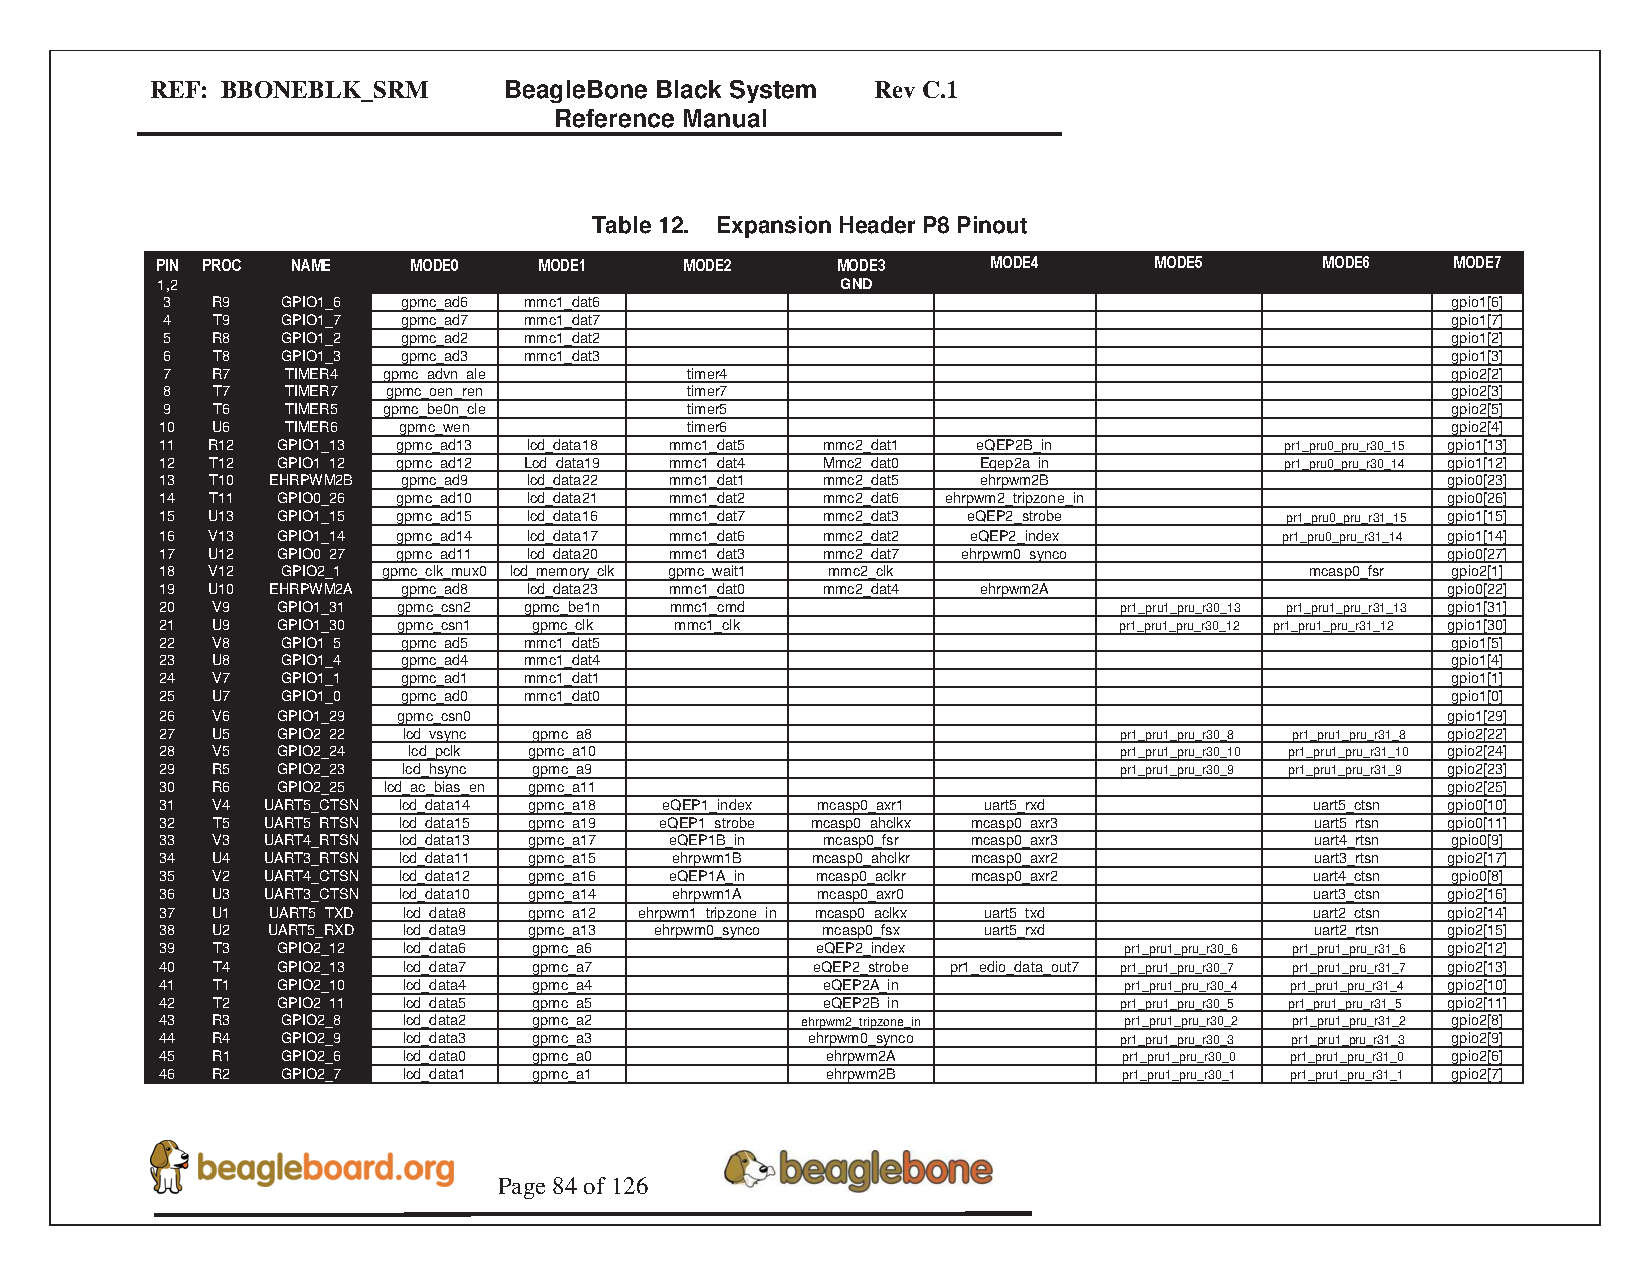
\includegraphics[page=1, height=0.4\textheight]{./Resources/tabela_pinos_SRM.pdf}
			\end{center}
		\end{table}
		%\includegraphics[page=3, scale=0.5]{./Resources/BBB_SCH.pdf}
	\end{center}
\end{minipage}

%tabela do header 9
\begin{minipage}[b][.49\textheight]{1\textwidth}
	\begin{center}
		\begin{table}[H]
			\captionsetup{justification=centering}
			\caption[Lista de pinos do \textit{header} P9 e seus respectivos modos de funcionamento]{Lista de pinos do \textit{header} P9 e seus respectivos modos de funcionamento \\ fonte: COLEY}
			\label{p9-header}
			\begin{center}
				\includegraphics[page=2, height=0.4\textheight]{./Resources/tabela_pinos_SRM.pdf}
			\end{center}
		\end{table}
		%\includegraphics[page=3, scale=0.5]{./Resources/BBB_SCH.pdf}
	\end{center}
\end{minipage}

%P�ginas relevantes do manual do SoC
%1356 - pullup, RXactive, etc e 1365 - registers offset, 1422 - registrador


\section{\textit{Device-tree}}
A \textit{Device Tree} ou DT � basicamente uma estrutura de dados utilizada para descrever \textit{hardware}, cujo objetivo � possibilitar que as caracter�sticas de \textit{hardware} de um sistema espec�fico sejam passadas para o SO durante o \textit{boot}, ao inv�s de estas informa��es ficarem gravadas no SO \cite{devicetree}, o que possibilita que um \textit{driver} do Kernel seja usado em configura��es diferentes de \textit{hardware} sem a necessidade de modifica��es em seu c�digo-fonte. Com rela��o aos sistemas equipados com processadores \textit{advanced risc machine} (ARM), a necessidade de uso da DT surgiu devido ao grande n�mero de novas placas, que tornou muito dif�cil manter uma vers�o do Kernel para cada sistema. Seu objetivo n�o � modificar o sistema em tempo de execu��o, por�m no caso da BBB, foi criada uma solu��o chamada \textit{Device Tree Overlay} (ou sobreposi��o) para executar esta fun��o, facilitando a configura��o de GPIO, dentre outras fun��es, e uso da DT pelo usu�rio final \cite{bbb_devicetree}, fatores que s�o do interesse de aprendizes da �rea.

Uma DT � uma estrutura em �rvore, composta de n�s e propriedades. Uma abordagem para entender o seu funcionamento � por meio de um exemplo de sobreposi��o espec�fico para a BBB. Na caixa de c�digo-fonte \ref{dt_example} � apresentado um exemplo de sobreposi��o de DT espec�fico da BBB que apresenta os principais conceitos para o uso desta ferramenta.

Neste c�digo, na linha 14 � definida a plataforma � qual esta DT se refere. Com isso, ficam declaradas as funcionalidades de \textit{hardware} do sistema. Na sequ�ncia, a identifica��o mostra quais sobreposi��es de DT est�o carregadas e o nome do arquivo compilado deve ser igual ao nome nela atribu�do; a vers�o deve ser 00A0 para a BBB. Entre as linhas 20 e 26 s�o listados os recursos de \textit{hardware} utilizados por esta sobreposi��o, que impedem que outras sobreposi��es que usem os mesmos recursos sejam carregadas; no caso deste exemplo, os pinos referentes � UART1, assim como o pr�prio dispositivo UART1 s�o utilizados. A seguir, os fragmentos descrevem qual dispositivo ter� suas configura��es sobrepostas. No fragmento 0, � o multiplexador dos pinos da BBB, compat�vel com o \textit{driver} \textit{pinctrl-single} - os dois valores hexadecimais utilizados para cada pino s�o o \textit{offset} do pino com rela��o ao seu registrador e a configura��o do pino. J� no fragmento 1 � configurada a interface UART1. Por enquanto, ser�o introduzidas somente as quest�es referentes � configura��o do multiplexador, uma vez que seu conhecimento foi necess�rio para o uso dos pinos no modo GPIO.

Para determinar o valor hexadecimal de \textit{offset} do pino ao qual se deseja aplicar uma configura��o, primeiro � preciso obter seu nome a partir do seu n�mero na barra de pinos, conforme ilustrado na figura \ref{bbb_pins_def}, consultando as tabelas \ref{p8-header} e \ref{p9-header}, nas quais o nome do pino � referente ao \textbf{modo 0}, que tamb�m � o nome do pino no manual do SoC \cite{bbb_srm, soc_manual}. A seguir, obt�m-se o valor hexadecimal do registrador referente ao pino, na tabela \ref{dt_offset} presente no anexo \ref{Anexo2}, adaptada do manual do SoC, e subtrai-se 0x800 de seu valor original.

\lstset{language=dtc}
\begin{lstlisting}[frame=single, basicstyle=\linespread{0.85}\ttfamily, caption=Sobreposi��o de \textit{device tree}, label=dt_example]
/* Copyright (C) 2013 CircuitCo */
/dts-v1/;
/plugin/;

/ {
	compatible = "ti,beaglebone", "ti,beaglebone-black";

	/* identification */
	part-number = "BB-UART1";
	version = "00A0";
	
	/* state the resources this cape uses */
	exclusive-use =
		/* the pin header uses */
		"P9.24",        /* uart1_txd */
		"P9.26",        /* uart1_rxd */
		/* the hardware ip uses */
		"uart1";
	
	fragment@0 {
		target = <&am33xx_pinmux>;
		__overlay__ {
			bb_uart1_pins: pinmux_bb_uart1_pins {
				pinctrl-single,pins = <
		/* P9.24 uart1_txd.uart1_txd MODE0 OUTPUT (TX) */
					0x184 0x20
		/* P9.26 uart1_rxd.uart1_rxd MODE0 INPUT (RX) */ 
					0x180 0x20
				>;
			};
		};
	};
	
	fragment@1 {
		target = <&uart2>;	/* really uart1 */
		__overlay__ {
			status = "okay";
			pinctrl-names = "default";
			pinctrl-0 = <&bb_uart1_pins>;
		};
	};
};
\end{lstlisting}

%\newpage

Com rela��o � configura��o do pino, este aceita os par�metros de ajuste de \textit{slew-rate}, ativa��o do \textit{buffer} de entrada, ajuste e ativa��o do \textit{pull-up/pull-down} interno e sele��o do modo de opera��o do pino. Note-se que, com rela��o ao buffer de entrada, ao menos um blog da internet refere-se a este bit como sendo um bit de sele��o para entrada \textbf{ou} sa�da \cite{derek_devtree}, por�m o manual indica que quando o bit est� setado, o pino pode ser usado tanto como entrada quanto sa�da \cite{soc_manual}. A tabela \ref{pad_cfg} apresenta os campos do registrador de controle de E/S, assim como a descri��o de cada campo e os valores aceitos.

\begin{center}
	\begin{table}[H]
		\captionsetup{justification=centering}
		\caption[Descri��o dos campos do registrador de controle de \textit{pads}]{Descri��o dos campos do registrador de controle de \textit{pads}. \\Fonte: adaptado de TEXAS INSTRUMENTS(2014)}
		\label{pad_cfg}
		\begin{tabular}{ | M{1cm} | M{3cm} | M{1cm} | M{10cm} |}
			\hline
			\textbf{Bit} & \textbf{Campo} & \textbf{Valor} & \textbf{Descri��o} \\ \hline
			31-7 & Reservado &  & Reservado. Leitura retorna 0 \\ \hline
			6 & SLEWCTRL & \shortstack{ \quad \\ 0 \\ 1} & \shortstack{Seleciona entre \textit{slew-rate} r�pido ou lento \\ 0 - r�pido \\ 1 - lento} \\ \hline
			5 & RXACTIVE & \shortstack{ \quad \\ 0 \\ 1} & \shortstack{Ativa modo de entrada para o pino \\ 0 - somente sa�da \\ 1 - Receptor ativado. Entrada ou sa�da}. \\ \hline
			4 & PULLTYPESEL & \shortstack{ \quad \\ 0 \\ 1} & \shortstack{Sele��o de pull-up/pull-down \\ 0 - pull-down \\ 1 - pull-up} \\ \hline
			3 & PULLUDEN & \shortstack{ \quad \\ 0 \\ 1} & \shortstack{Habilita pull-up/pull-down \\ 0 - habilitado \\ 1 - desabilitado} \\ \hline
			2-0 & MUXMODE & 0-7 & Sele��o de funcionalidade do pino multiplexado \\ \hline
		\end{tabular}
	\end{table}
\end{center}

%\newpage

\begin{comment}
%tabela do header 8
\begin{minipage}[t][.49\textheight]{1\textwidth}
	\begin{center}
		\begin{table}[H]
			\captionsetup{justification=centering}
			\caption[Lista de pinos do \textit{header} P8 e seus respectivos modos de funcionamento]{Lista de pinos do \textit{header} P8 e seus respectivos modos de funcionamento \\ Fonte: COLEY (2014)}
			\label{p8-header}
			\begin{center}
				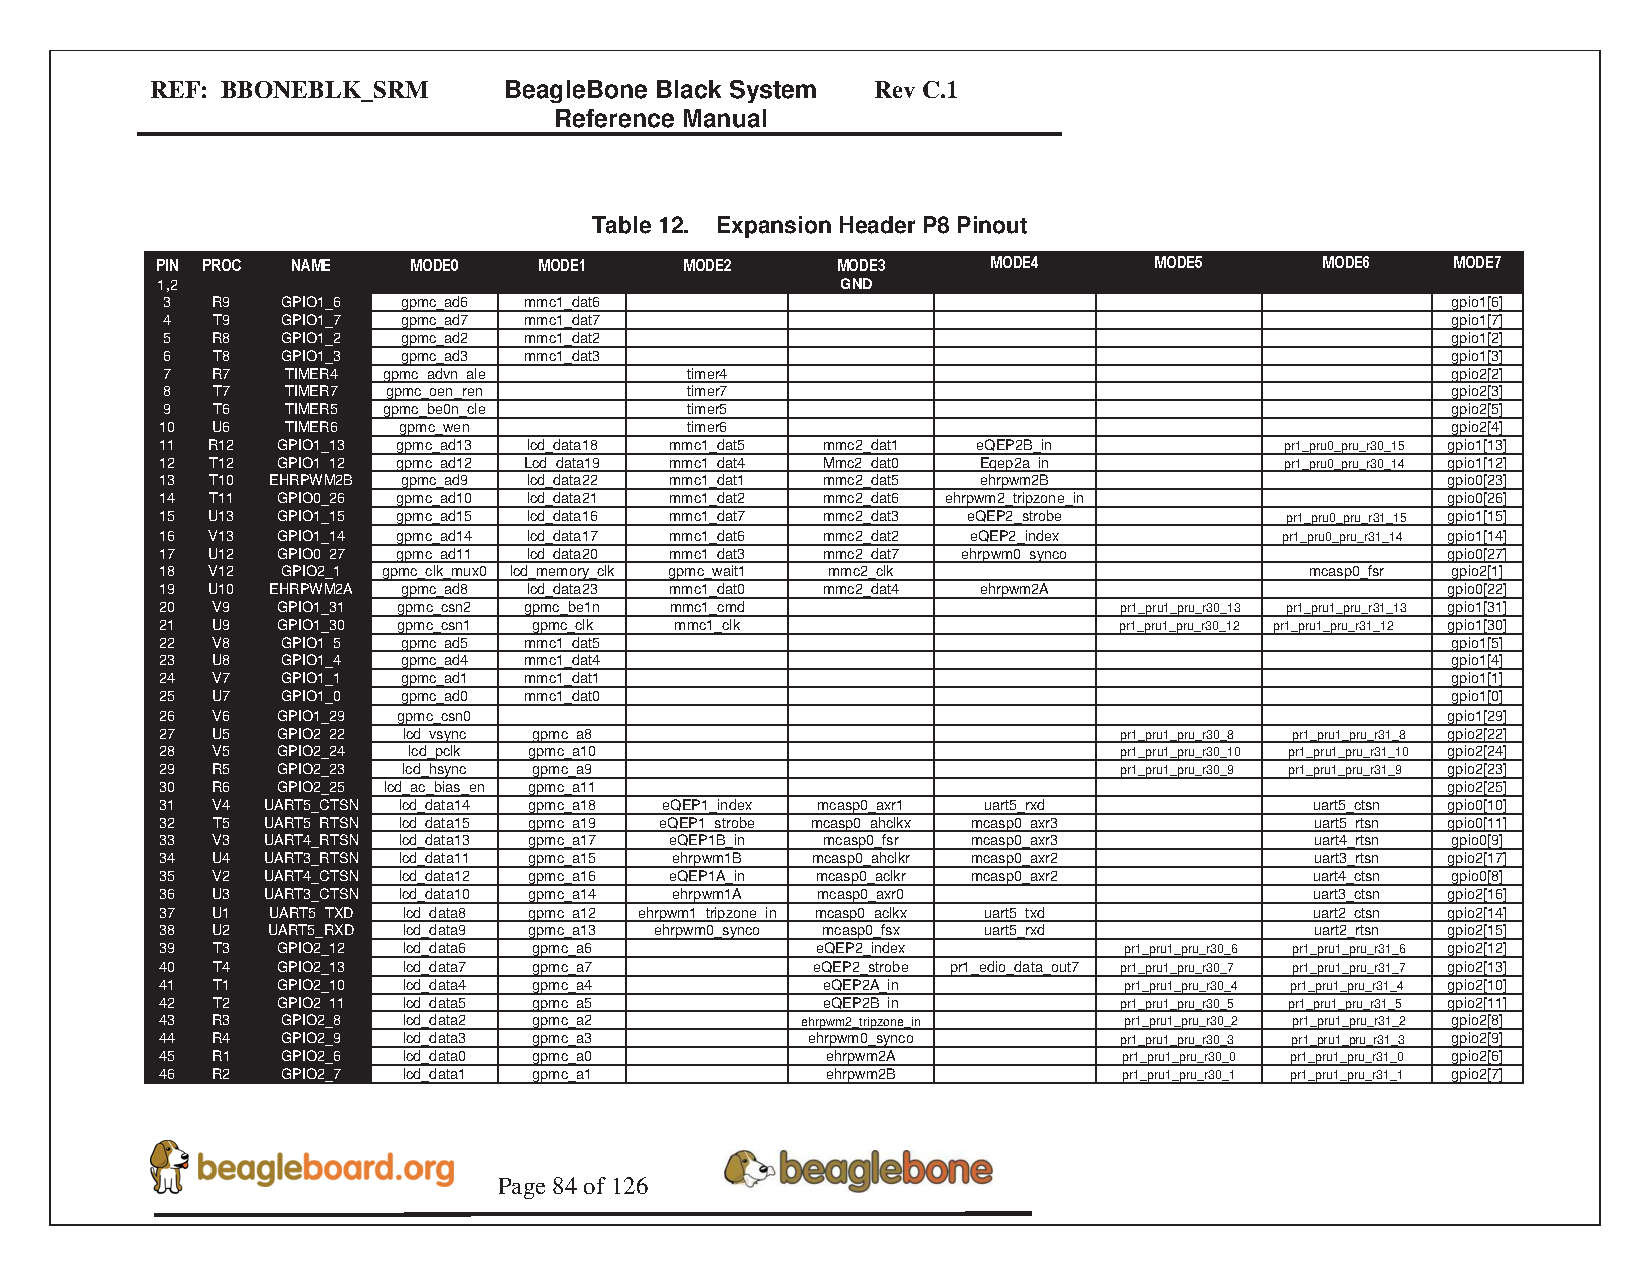
\includegraphics[page=1, height=0.5\textheight]{./Resources/tabela_pinos_SRM.pdf}
			\end{center}
		\end{table}
		%\includegraphics[page=3, scale=0.5]{./Resources/BBB_SCH.pdf}
	\end{center}
\end{minipage}
\end{comment}
%\newpage

\begin{comment}
%tabela do header 9
\begin{minipage}[b][.49\textheight]{1\textwidth}
	\begin{center}
		\begin{table}[H]
			\captionsetup{justification=centering}
			\caption[Lista de pinos do \textit{header} P9 e seus respectivos modos de funcionamento]{Lista de pinos do \textit{header} P9 e seus respectivos modos de funcionamento \\ Fonte: COLEY (2014)}
			\label{p9-header}
			\begin{center}
				\includegraphics[page=2, height=0.5\textheight]{./Resources/tabela_pinos_SRM.pdf}
			\end{center}
		\end{table}
		%\includegraphics[page=3, scale=0.5]{./Resources/BBB_SCH.pdf}
	\end{center}
\end{minipage}
\end{comment}

%P�ginas relevantes do manual do SoC
%1356 - pullup, RXactive, etc e 1365 - registers offset, 1422 - registrador

\label{dt_section}

%\subsection{Programa��o em Python}

\section{Programa��o em Node.js (Javascript)}
Node.js � um ambiente em tempo de execu��o recente, criado em 2009 \cite{node_created},que permite a execu��o no servidor de programas escritos em Javascript. Para tal, este ambiente utiliza um motor implementado pelo Google para seu navegador Chrome --- o \textit{V8}, que compila o Javascript em c�digo de m�quina e n�o \textit{bytecode} ou interpreta��o \textit{on-the-fly}, o que torna a execu��o de Javascript extremamente r�pida \cite{node_fast}, embora seja importante lembrar que o \textit{overhead} inerente de lingaugens de tipagem din�mica custa o tempo de processamento de resolu��o do tipo de vari�vel utilizada \cite{node_dyntype}. 

Node, devido � natureza ass�ncrona de I/O do Javascript, implementa um suporte nativo � programa��o orientada a eventos, ainda que seja executado em uma �nica \textit{thread}, o que o torna um diferencial com rela��o �s outras lingaugens de programa��o mais populares, que exigem do desenvolvedor a implementa��o de processos de \textit{multithreading} para atingir paralelismo de processamento \cite{node_intro}. Ainda, o estilo de programa��o em Node � orientado a \textit{callbacks}, que nada mais � do que passar como argumento uma fun��o que ser� executada assim que um evento acabar.

Historicamente, o desenvolvimento de \textit{multithreading} surgiu da necessidade de servi�os de rede que possibilitassem m�ltiplas comunica��es em paralelo, o que � conhecido como m�ltiplas fontes de I/O e assim ser� referenciado neste trabalho --- isto ocorreu devido ao fato de linguagens tradicionais de programa��o, mais antigas, focarem na implementa��o de aplica��es operadas por um �nico ser humano enquanto, com o desenvolvimento da internet, esta realidade mudou drasticamente, exigindo processamento de I/O massivo \cite{node_book}. Em processadores com diversos n�cleos, isso significa processamento em paralelo, enquanto em processadores com um �nico n�cleo � implementada uma multiplexa��o temporal que permite tal t�cnica. O fato mais not�vel das implementa��es de \textit{multithreading} � a complexidade do c�digo, que n�o � trivial e geralmente d� origem a c�digos mal estruturados e repletos de vari�veis globais, dif�ceis de manter \cite{node_intro, node_book}.

Javascript, que nasceu como uma linguagem para execu��o no cliente, tornou-se a espinha dorsal de aplica��es HTML modernas e, recentemente, ficou muito popular dentre aplica��es no servidor. Especificamente em Node, o comportamento ass�ncrono � a regra geral, devido � orienta��o a eventos. Isto leva programadores acostumados a linguagens s�ncronas como C a terem dificuldades iniciais de programa��o: o uso de \textit{callbacks} de evento � fundamental para estruturar a ordem com que certas tarefas s�o executadas, sempre ap�s o final do evento pai \cite{node_book}. � importante salientar que este tipo de implementa��o ocorre de forma transparente ao usu�rio mas, na verdade, nada mais � do que um \textit{loop} principal cujo objetivo � cuidar de todas as chamadas a fun��es. Outro ponto not�vel relacionado ao Node � que, para executar aplica��es em m�ltiplos n�cleos, � preciso executar m�ltiplas inst�ncias, o que pode ser gerenciado com bibliotecas de suporte \cite{node_intro, node_book}. Note-se tamb�m que os termos \textit{orientado a eventos} e \textit{ass�ncrono} s�o equivalentes \cite{node_book}.

Para ilustrar o comportamento ass�ncrono do Node, no c�digo a seguir n�o h� garantia alguma de que a fun��o executada na segunda linha receba um par�metro diferente de nulo (Null) \cite{node_book}:

\lstset{language=javascript}
\begin{lstlisting}[frame=single, basicstyle=\linespread{0.85}\ttfamily]
var botaoStatus = leBotao();
imprimeValorBotao(botaoStatus); //nao ha garantia de que leBotao ja acabou de ser executada
\end{lstlisting}

A maneira correta para executar este tipo de c�digo seria usando uma fun��o de callback, como descrito no trecho de c�digo abaixo, embora esta n�o seja a �nica maneira de faz�-lo. Observe-se que a fun��o � declarada como um par�metro de \textit{leBotao} e n�o tem nome --- � uma fun��o an�nima. Embora isto seja pr�tico, do ponto de vista de manuten��o de c�digo e \textit{debug} � uma pr�tica que deve ser evitada \cite{callback_hell, avoid_hell}.

\lstset{language=javascript}
\begin{lstlisting}[frame=single, basicstyle=\linespread{0.85}\ttfamily]
leBotao(function(botaoStatus){
	imprimeValorBotao(botaoStatus); //so acontece depois que o botao eh lido
});
\end{lstlisting}

\subsection{\textit{Node Package Manager - NPM}}

O \textit{Node Package Manager}, ou simplesmente NPM, � n�o somente um gerenciador de pacotes como tamb�m � um reposit�rio de pacotes de terceiros e um padr�o para defini��o de depend�ncias. Os pacotes ficam em um registro p�blico e podem ser gerenciados por uma ferramenta pr�pria por linha de comando. O uso do NPM n�o � obrigat�rio, mas � medida que aplica��es mais complexas s�o desenvolvidas � quase mandat�rio seu uso, pois assim � poss�vel usar m�dulos prontos para executar diversas tarefas com facilidade. Uma vantagem do NPM � que os m�dulos podem ser instalados localmente, restringindo-os ao diret�rio do projeto e, portanto, garantindo certo n�vel de seguran�a. \cite{node_book}. Abaixo � apresentado um exemplo no qual o pacote fict�cio \textit{meuPacote} � instalado para a vers�o mais recente adicionada ao reposit�rio do NPM:

\lstset{language=bash}
\begin{lstlisting}[frame=single, basicstyle=\linespread{0.85}\ttfamily]
npm install meuPacote@latest
\end{lstlisting}

Outro exemplo de uso do NPM � a defini��o de depend�ncias de um projeto e posterior possibilidade de instala��o de todas elas de uma s� vez. Para isto, um arquivo no formato JSON descreve estas depend�ncias e outras informa��es do projeto:

\lstset{language=javascript}
\begin{lstlisting}[frame=single, basicstyle=\linespread{0.85}\ttfamily]
{
	"name" : "meuPacote",
	"version" : "1.0.0",
	"dependencies" : {
		"debug" : "0.3.x",
		"nano" : "*",
		"request" : ">0.2.0"
	}
}
\end{lstlisting}

E a instala��o das depend�ncias se d� da seguinte maneira, assumindo que o presente diret�rio de trabalho � o mesmo do projeto:

\lstset{language=bash}
\begin{lstlisting}[frame=single, basicstyle=\linespread{0.85}\ttfamily]
npm install
\end{lstlisting}

\subsection{\textit{MEAN Stack}}

MEAN � uma pilha de desenvolvimento, de c�digo aberto, para aplica��es web e prov� um conjunto de quatro ferramentas que, juntas, s�o a base necess�ria para a cria��o de aplica��es tanto de servidor quanto do cliente. Um exemplo de pilha de desenvolvimento para aplica��es web muito disseminado � a pilha LAMP. Voltando � MEAN, cada uma das 4 letras deste acr�nimo representa uma das ferramentas \cite{node_mean}:

\begin{itemize}
	\item \textbf{MongoDB} - banco de dados orientado a objetos
	\item \textbf{Express.js} - framework para cria��o de servidor web e roteamento
	\item \textbf{Angular.js} - framework para aplica��es web
	\item \textbf{Node.js} - base da aplica��o do servidor
\end{itemize}

Note-se que toda a pilha � baseada na linguagem Javascript, o que permite ao desenvolvedor de uma solu��o completa uma curva de aprendizado mais r�pida, pois menos tempo � empregado aprendendo a sintaxe e o paradigma de programa��o e mais tempo dedicado � funcionalidade da aplica��o em si \cite{node_mean}.

\subsection{Servidor Express.js}

Express � um framework de \textit{middleware} para implementa��o de aplica��es web no servidor, incluindo mas n�o limitado a roteamento e opera��es HTTP, a exemplo dos m�todos GET e POST. Embora o Node apresente um m�dulo dedicado a HTTP, a proposta do Express � simplificar seu uso e evitar que o mesmo trabalho seja realizado m�ltiplas vezes e por v�rias pessoas diferentes \cite{node_mean}.

Dentre as facilidades proporcionadas pelo node est� a f�cil implementa��o de diferentes respostas para diferentes tipos de requisi��es baseadas no m�todo HTTP e a renderiza��o din�mica de documentos HTML \cite{node_book}. O tratamento de requisi��es baseadas no m�todo HTTP, possibilitado pelo Express, tamb�m � conhecido como RESTful API, que � uma API baseada no REST (\textit{Representational State Transfer}). Este por sua vez � um modelo para servi�os web que implementa as opera��es HTTP POST, GET, PUT e DELETE, que s�o mapeadas como opera��es b�sicas de banco de dados: criar, ler, atualizar e deletar \cite{node_mean}.

%\subsection{Performance do Node.js}

%\subsection{Intera��o com c�digo escrito em C/C++}

%\subsection{Confiabilidade e seguran�a quanto ao uso de m�dulos de terceiros}


%\section{Computa��o em nuvem e Internet das Coisas}

\section{Circuitos de Interface}
No �mbito deste trabalho, circuitos de interface s�o circuitos eletr�nicos que possibilitaram a intera��o entre a plataforma BeagleBone Black e os sensores e atuadores do sistema mec�nico. O projeto adequado destes circuitos foi essencial n�o somente para que o projeto funcionasse corretamente, mas tamb�m para evitar que componentes do sistema, a exemplo da BBB, fossem danificados. Nesta se��o, ser� abordada a teoria essencial para o projeto destes, desde conceitos relacionados � teoria de sinais, passando por alguns elementos b�sicos da eletr�nica e finalizando com as caracter�sticas dos sensores e atuadores empregados.

\subsection{Sinais}

Sinais s�o fun��es matem�ticas que guardam informa��es acerca de fen�menos f�sicos, a exemplo da temperatura de um elemento em fun��o do tempo ou a representa��o do som de um instrumento musical. Na figura \ref{seno_1p} � apresentado um per�odo de um sinal senoidal puro. Uma vez que, para obter informa��es a partir de um sinal, � preciso process�-lo, as mais diversas grandezas f�sicas devem ser convertidas para grandezas manipul�veis pelo sistema de processamento --- que no caso de circuitos eletr�nicos � comumente a tens�o el�trica, embora outras grandezas tamb�m sejam utilizadas \cite{sedra}. Para que a convers�o de diferentes grandezas f�sicas em sinais el�tricos seja poss�vel, s�o empregados dispositivos sensores e transdutores.

\begin{figure}[H]
	\centering
	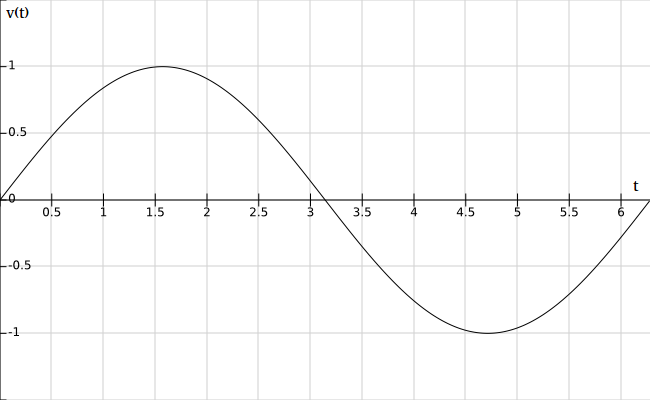
\includegraphics[scale=0.50]{./Resources/seno2.png}
	\captionsetup{justification=centering}
	\caption[Sinal senoidal em fun��o do tempo]{Sinal senoidal em fun��o do tempo}
	\label{seno_1p}
\end{figure}

\subsection{Dispositivos Semicondutores}

Diodos s�o os elementos eletr�nicos mais simples, constitu�dos de dois terminais que est�o conectados a uma jun��o PN, ou seja, a uma jun��o formada pelo contato entre dois cristais semicondutores dopados com impurezas de polaridades opostas \cite{juncoes_vero}. O efeito pr�tico desta jun��o � a capacidade de retifica��o: quando uma DDP positiva � aplicada aos terminais do diodo conforme exposto na figura \ref{diode}, a corrente el�trica flui pelos terminais do dispositivo e diz-se que o diodo est� polarizado diretamente; caso a DDP aplicada seja invertida, a corrente el�trica deixa de fluir pelo dispositivo \cite{sedra}. Este � considerado o diodo ideal, que � o modelo mais simplificado deste elemento e n�o leva em considera��o nenhuma caracter�stica real do mesmo.

\begin{figure}[H]
	\centering
	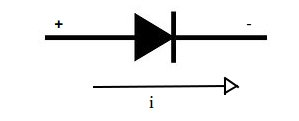
\includegraphics[scale=0.50]{./Resources/diode.jpg}
	\captionsetup{justification=centering}
	\caption[Representa��o esquem�tica do diodo polarizado diretamente]{Representa��o esquem�tica do diodo polarizado diretamente}
	\label{diode}
\end{figure}

O diodo ideal � descrito pela equa��o \ref{eq_diodo_real}, na qual $I_{s}$ � a corrente de satura��o reversa, $k=11600/\eta$, com $\eta$ igual a 1 para o germ�nio e 2 para o sil�cio e $T_{k}$ � a temperatura em kelvin. Muitas vezes, esta curva � aproximada por um modelo conhecido como \textit{circuito equivalente linear}, composto de um diodo em s�rie com uma fonte de tens�o e um resistor, que definem o limiar de condu��o e o n�vel de resist�ncia do dispositivo quando est� conduzindo \cite{boylestad}. A figura \ref{diodo_curva} ilustra um exemplo de curva do circuito equivalente a partir da representa��o real. Outra modelagem � conhecida como \textit{modelo para pequenos sinais}, no qual � fixado um ponto de opera��o em torno do qual a excurs�o do sinal aplicado ao circuito � pequena, conhecido como ponto de polariza��o ou \textbf{ponto quiescente}. Neste modelo, a regi�o exponencial � aproximada linearmente por um resistor cujo valor � o inverso da inclina��o da reta tangente ao ponto de polariza��o \cite{sedra}. Cabe salientar que o avan�o das ferramentas de computa��o tornaram poss�vel o c�lculo dos mais diversos circuitos eletr�nicos de forma r�pida e exata, relegando portanto os modelos simplificados a ferramentas de ensino ou para esbo�o de circuitos simples \cite{boylestad}, desde que os modelos empregados nas simula��es sejam fi�is ao comportamento real dos componentes \cite{sedra}.

\begin{equation}
	\label{eq_diodo_real}
	I_{d}=I_{s}\epsilon ^{kV_{d}/T_{k}}-I_{s}
\end{equation}

\begin{figure}[H]
	\centering
	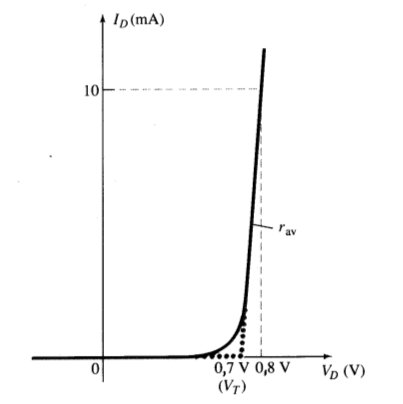
\includegraphics[scale=0.85]{./Resources/diodo_curva.jpg}
	\captionsetup{justification=centering}
	\caption[Defini��o do circuito equivalente linear, usando-se segmentos de reta para aproximar a curva caracter�stica]{Defini��o do circuito equivalente linear, usando-se segmentos de reta para aproximar a curva caracter�stica \\ Fonte: BOYLESTAD (2011)}
	\label{diodo_curva}
\end{figure}

A partir do conhecimento obtido com a introdu��o ao diodo e sua jun��o PN, ser� agora abordado o transistor bipolar de jun��o, tamb�m conhecido com BJT. De forma an�loga ao diodo, este dispositivo � constitu�do da jun��o de tr�s cristais semicondutores dopados, podendo ser uma jun��o do tipo NPN ou PNP: ambos funcionam de forma complementar, sendo que o tipo NPN conduz majoritariamente el�trons, enquanto o tipo PNP conduz majoritariamente lacunas. Na figura \ref{transistor} s�o apresentados os sentidos de corrente e os s�mbolos dos transistores PNP e NPN e, aplicando a lei das correntes de Kirchhoff, obt�m-se a rela��o entre as correntes de emissor, coletor e base do transistor, descritas pela equa��o \ref{eq_bjt_kirch} \cite{boylestad}. Note-se que � usado o sentido real da corrente e n�o o convencional, comumente adotado em c�lculos.

\begin{figure}[H]
	\centering
	\begin{subfigure}{.46\textwidth}
		\centering
		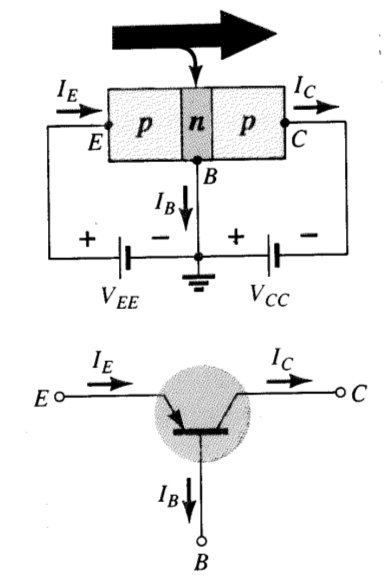
\includegraphics[height=8cm]{./Resources/bjt_pnp.jpg}
		\caption{Transistor \textit{pnp}}
		\label{transistor:1}
	\end{subfigure}
	\begin{subfigure}{.46\textwidth}
		\centering
		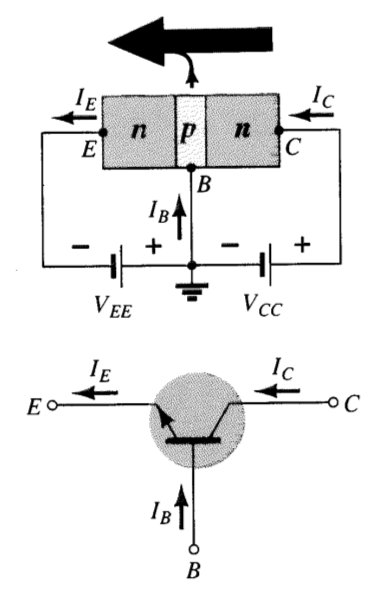
\includegraphics[height=8cm]{./Resources/bjt_npn.jpg}
		\caption{Transistor \textit{npn}}
		\label{transistor:2}
	\end{subfigure}
	\captionsetup{justification=centering}
	\caption[Nota��es e s�mbolos utilizados para a configura��o base-comum]{Nota��es e s�mbolos utilizados para a configura��o base-comum. \\Fonte: BOYLESTAD (2011)
	}
	\label{transistor}
\end{figure}

\begin{equation}
	\label{eq_bjt_kirch}
	I_{e}=I_{c} + I_{b}
\end{equation}

Para finalizar a introdu��o ao transistor bipolar, � apresentada uma rela��o simplificada entre as correntes de coletor $I_{c}$ e de base $I_{b}$ na equa��o \ref{eq_bjt_beta}, uma vez que esta � uma rela��o que permite a realiza��o de c�lculos r�pidos para esbo�ar circuitos com transistores BJT. Cabe salientar que a validade desta rela��o se d� somente quando o transistor est� corretamente polarizado e na regi�o de amplifica��o. Outro fato que deve ser levado em conta � que o valor de $\beta$ depende das caracter�sticas de constru��o de cada BJT e � um valor cujo desvio padr�o � elevado mesmo se comparados dois transistores reais do mesmo modelo \cite{boylestad}. Ainda que o conte�do relativo a transistores BJT seja muito mais extenso e detalhado, cabe ao leitor consultar as refer�ncias bilbiogr�ficas \cite{boylestad} e \cite{sedra} para mais detalhes acerca do tema. 

\begin{equation}
	\label{eq_bjt_beta}
	I_{c} = \beta\cdot I_{b}
\end{equation}

Existe outro tipo de transistor conhecido como transistor de efeito de campo ou FET. Embora este seja um dispositivo semelhante ao BJT no que diz respeito � aplica��o, ainda assim existem in�meras diferen�as entre eles, dentre as quais a mais not�vel � o fato de que o BJT � controlado a corrente, enquanto o FET � controlado a tens�o. Outra diferen�a importante � o fato de que transistores FET podem ser de canal \textit{n} ou canal \textit{p}, ou seja, s�o transistores unipolares --- que conduzem somente el�trons ou somente lacunas, respectivamente. Sendo um dispositivo controlado a tens�o, a imped�ncia de entrada � alt�ssima, muitas vezes considerada infinita em casos pr�ticos \cite{boylestad}. Uma subclasse destes dispositivos muito popular � o MOSFET - popularmente empregado como chave eletr�nica na �rea de circuitos integrados, mas tamb�m adotado para chaveamento de dispositivos de alta pot�ncia em fun��o da sua baixa imped�ncia quando ligado \cite{sedra}. O s�mbolo dos transistores JFET e MOSFET s�o apresentados na figura \ref{fet_symbol}. Os terminais do dispositivo s�o nomeados \textit{fonte} (\textit{source}), \textit{dreno} (\textit{drain}) e \textit{porta} (\textit{gate}).

\begin{figure}[H]
	\centering
	\begin{subfigure}{.23\textwidth}
		\centering
		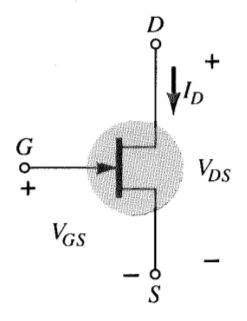
\includegraphics[height=5cm]{./Resources/fet_n.jpg}
		\caption{FET canal \textit{n}}
		\label{fet_symbol:1}
	\end{subfigure}
	\begin{subfigure}{.23\textwidth}
		\centering
		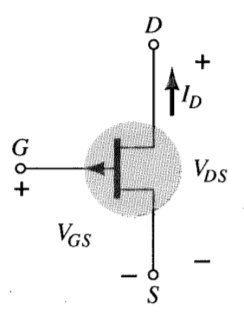
\includegraphics[height=5cm]{./Resources/fet_p.jpg}
		\caption{FET canal \textit{p}}
		\label{fet_symbol:2}
	\end{subfigure}
	\begin{subfigure}{.23\textwidth}
		\centering
		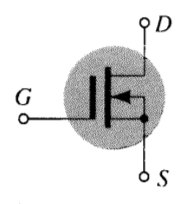
\includegraphics[height=3cm]{./Resources/mosfet_n.jpg}
		\caption{MOSFET canal \textit{n}}
		\label{fet_symbol:3}
	\end{subfigure}
	\begin{subfigure}{.23\textwidth}
		\centering
		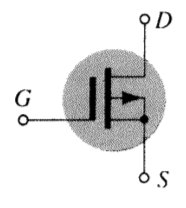
\includegraphics[height=3cm]{./Resources/mosfet_p.jpg}
		\caption{MOSFET canal \textit{p}}
		\label{fet_symbol:4}
	\end{subfigure}
	\captionsetup{justification=centering}
	\caption[S�mbolos do JFET e do MOSFET]{S�mbolos do JFET e do MOSFET. \\Fonte: BOYLESTAD (2011)}
	\label{fet_symbol}
\end{figure}

Os transistores do tipo FET/MOSFET s�o tamb�m conhecidos como resistores controlados por tens�o, o que ajuda a entender seu funcionamento: assumindo que h� uma DDP entre os terminais de \textit{dreno} e \textit{fonte} $V_{ds}$, a resist�ncia � passagem de corrente por estes terminais � controlada pela tens�o aplicada � \textit{porta} com rela��o � \textit{fonte} $V_{gs}$ do dispositivo. Quanto mais pr�ximo de zero � a tens�o, maior � o valor da resist�ncia, para os dispositivos FET e MOSFET intensifica��o \cite{boylestad}. Este comportamento � ilustrado na figura \ref{curva_fet} e a equa��o simplificada \ref{eq_fet_id} rege o comportamento de $I_{d}$ em fun��o de $V_{gs}$, na qual $I_{dss}$ e $V_{p}$ s�o os pontos not�veis no gr�fico da figura \ref{curva_fet} \cite{boylestad}.

De maneira an�loga ao BJT, tanto o FET quanto suas varia��es, aperfei�oamentos e aplica��es possuem uma teoria vasta, que n�o cabe a este trabalho detalhar. Para o aprofundamento no tema, recomenda-se a leitura da bilbiografia --- em especial de \cite{boylestad} e \cite{sedra}.

\begin{figure}[H]
	\centering
	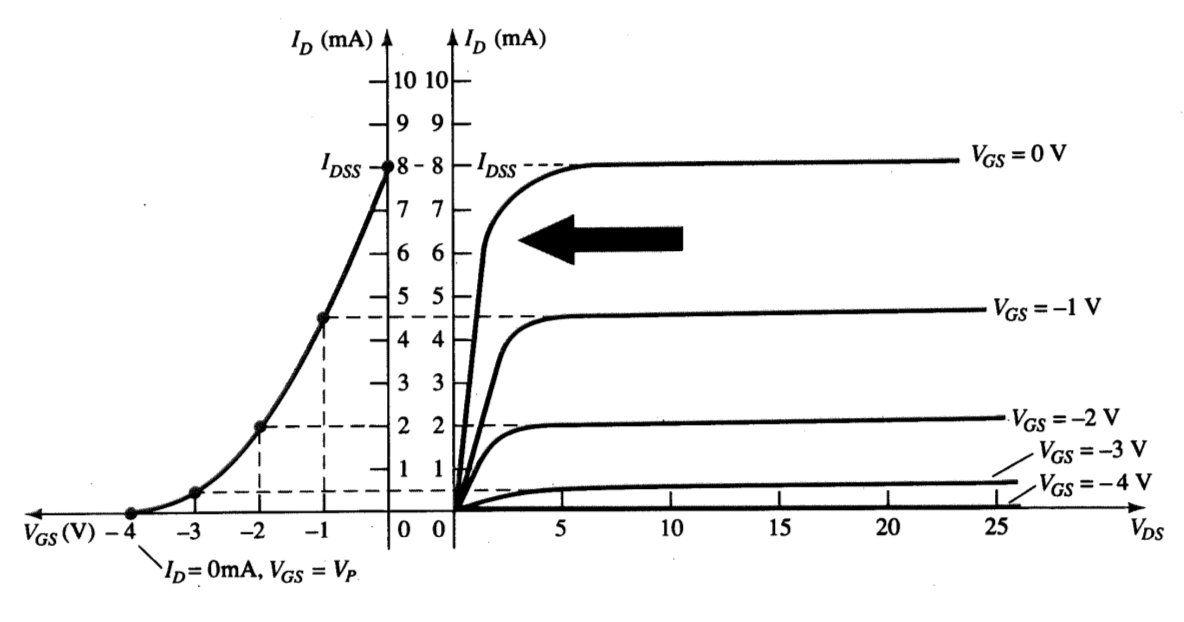
\includegraphics[scale=0.38]{./Resources/curva_fet.jpg}
	\captionsetup{justification=centering}
	\caption[Obtendo a curva de transfer�ncia das curvas de dreno de um JFET]{Obtendo a curva de transfer�ncia das curvas de dreno \\ Fonte: BOYLESTAD (2011)}
	\label{curva_fet}
\end{figure}

\begin{equation}
	\label{eq_fet_id}
	I_{d} = I_{dss} \left(1 - \frac{V_{gs}}{V_{p}}\right)^2
\end{equation}

\subsection{Sensor de temperatura DS18B20}

O sensor de temperatura DS18B20, projetado pela Maxim, � um sensor digital que utiliza somente um pino de dados para comunica��o com o dispositivo \textit{master}, cujas regras s�o estabelecidas pelo protocolo propriet�rio de comunica��o $\textit{1-Wire}^\textregistered$ \cite{ds18b20}.

\textit{1-Wire} � um protocolo de comunica��o serial \textit{half-duplex} que utiliza uma linha para transmiss�o de dados, al�m da refer�ncia. Ele � do tipo \textit{master/slave}, ou seja, um dispositivo \textit{master} inicia a comunica��o e os dispositivos \textit{slave} somente respondem aos seus comandos. No caso deste protocolo espec�fico, todo dispositivo possui um identificador de 64 bits �nico, dentro do qual um byte indica o tipo do dispositivo. Devido ao seu modo de funcionamento, quando a linha de dados � desconectada, os dispositivos \textit{slave} entram em estado de \textit{reset}, o que favorece seu uso em aplica��es de contato. Enquanto a maioria destes dispositivos tem uma faixa de alimenta��o de 2,80-5,25V e n�o possui pino para alimenta��o \cite{onewire_ov} -- utilizando um sistema de alimenta��o parasita -- o sensor DS18B20 tem a possibilidade de alimenta��o parasita ou n�o e sua faixa tolerada para funcionamento � de 3-5,5V \cite{ds18b20}.

Uma vez que este protocolo de comunica��o foi concebido para opera��es nas quais os dispositivos \textit{master} e \textit{slave} est�o fisicamente muito pr�ximos, alguns cuidados devem ser observados ao utilizar linhas de transmiss�o de longas dist�ncias para manter a boa performance do sistema \cite{onewire_distance}. Como o estudo da Maxim acerca das implica��es do uso de linhas de longa dist�ncia negligencia este aspecto para redes com poucos dispositivos e cabeamento curto (menor que 10m), os cuidados de projeto das redes \textit{1-wire} n�o ser�o aqui especificados, deixando um aviso para trabalhos futuros que visem aplica��es de longas dist�ncias ou com n�mero elevado de dispositivos, a exemplo de uma microcervejaria de porte industrial.

Com rela��o a aspectos espec�ficos do sensor de temperatura, este apresenta precis�o de 0,5\si{\degree}C para a faixa de temperaturas de -10\si{\degree}C a +85\si{\degree}C, e de 2,0\si{\degree}C para a faixa completa de opera��o, de -55\si{\degree}C a +125\si{\degree}C. Quanto � resolu��o, esta pode ser programada de 9 a 12 bits, sendo 8 bits para a parte inteira e 1 a 4 bits decimais. O custo da melhor resolu��o � o aumento no tempo de convers�o de uma leitura para valor digital, variando de 93,75ms a 750ms para os casos extremos \cite{ds18b20}.

A arquitetura interna do CI � apresentada na figura \ref{18b_blocos}. Nota-se que o dispositivo, por utilizar o protocolo \textit{1-Wire}, tem uma ROM de 64 bits para identifica��o \cite{onewire_ov}, al�m de uma regi�o de mem�ria de rascunho, que consiste de uma mem�ria SRAM de 64 bits, dividida em 8 regi�es de 1 byte, para promover a interface com as funcionalidades do CI: sensor de temperatura, alarmes program�veis para estouro de valores m�nimo e m�ximo das medi��es, registrador de configura��o da resolu��o e gerador de c�digo CRC de 8 bits \cite{ds18b20}. A figura \ref{18b_mmap} apresenta o mapa de mem�ria do DS18B20 -- nota-se que os registradores de configura��o e alarme s�o copiados para uma mem�ria n�o vol�til (EEPROM) ap�s configurados pelo \textit{master}, retendo seus valores mesmo em caso de corte na alimenta��o. Outra informa��o �til obtida a partir da figura \ref{18b_mmap} � o valor da temperatura lido ap�s uma queda de alimenta��o, que � de +85\si{\degree} C at� que o dispositivo esteja pronto para uso \cite{ds18b20}.

\begin{figure}[H]
	\centering
	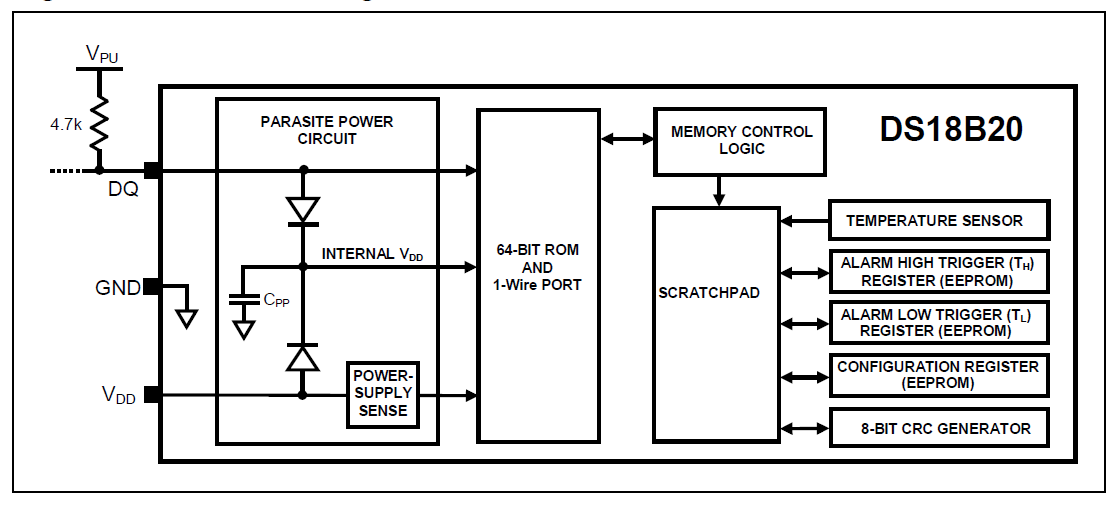
\includegraphics[width=12cm]{./Resources/ds18b20-blocos.png}
	\captionsetup{justification=centering}
	\caption[Arquitetura interna do DS18B20]{Arquitetura interna do DS18B20 \\Fonte: MAXIM INTEGRATED
	}
	\label{18b_blocos}
\end{figure}

\begin{figure}[H]
	\centering
	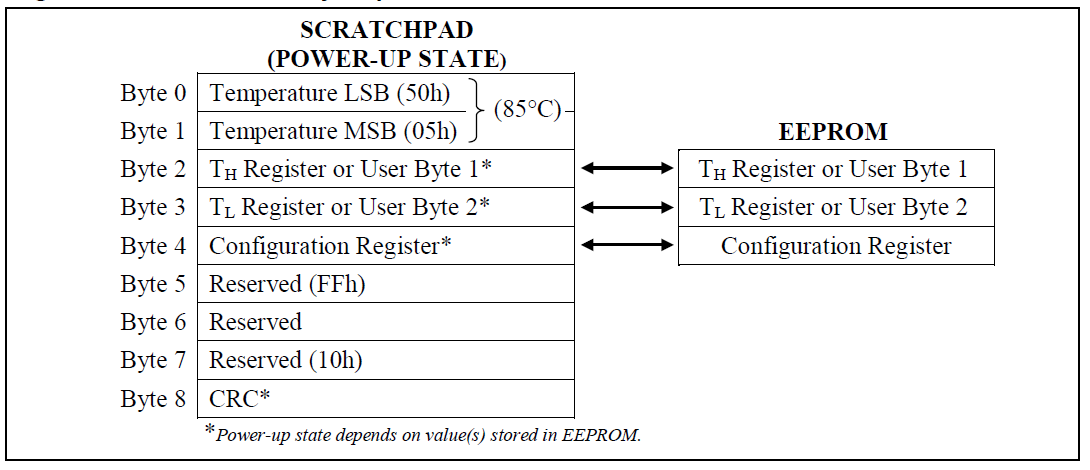
\includegraphics[width=11.83cm]{./Resources/ds18b20-mmap.png}
	\captionsetup{justification=centering}
	\caption[Mapa de mem�ria do DS18B20]{Mapa de mem�ria do DS18B20. \\Fonte: MAXIM INTEGRATED
	}
	\label{18b_mmap}
\end{figure}

As leituras de temperatura s�o feitas em dois bytes, LSB e MSB, representados na figura \ref{18b_formato}, e que juntos s�o uma representa��o em complemento de dois, sendo que os 5 bits mais significativos s�o redundantes e, para resolu��es menores do que 12 bits, o valor dos bits menos significativos � indefinido (1 bit indefinido para 11 bits de resolu��o; 2 bits indefinidos para 10 bits de resolu��o, etc).

\begin{figure}[H]
	\centering
	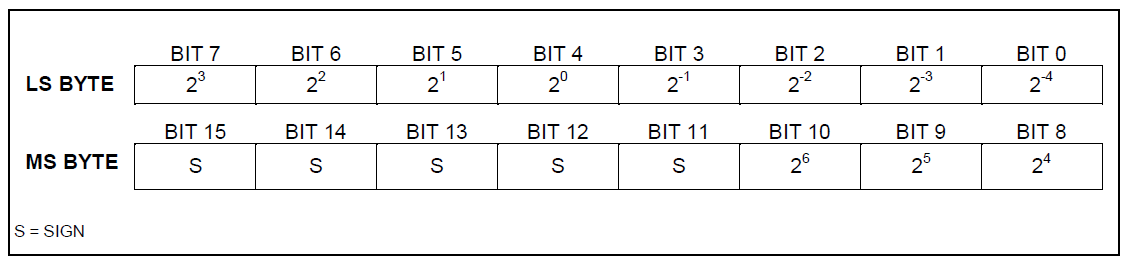
\includegraphics[width=11.83cm]{./Resources/ds18b20-formato.png}
	\captionsetup{justification=centering}
	\caption[Registradores de temperatura do DS18B20]{Registradores de temperatura do DS18B20. \\Fonte: MAXIM INTEGRATED
	}
	\label{18b_formato}
\end{figure}

O Kernel do Linux possui \textit{device drivers} que suportam parcialmente o uso do sensor DS18B20, portanto n�o h� a necessidade de descrever em detalhes o protocolo \textit{1-Wire}. O \textit{device driver} \textit{w1-gpio} controla o barramento (\textit{master}) \textit{1-wire} utilizando a API GPIO para controlar a linha, sendo que a porta utilizada � especificada na descri��o de hardware do sistema embarcado (\textit{device tree}) abordada na se��o \ref{dt_section}. O \textit{device driver} \textit{w1-therm} suporta algumas fam�lias de sensores de temperatura da Maxim (\textit{slave}), dentre elas a DS18*20, fazendo convers�es b�sicas de temperatura e fornecendo-as ao sistema por meio do FS (\textit{File System} ou Sistema de Arquivos). O resultado da abertura e leitura do arquivo correspondente a um sensor, � a convers�o de temperatura pelo \textit{driver} e posterior fornecimento dos dados recebidos do sensor --- status da checagem do CRC e temperatura em \si{\degree}C/1000. Este driver n�o suporta convers�o de temperatura simult�nea de m�ltiplos sensores nem redu��o da precis�o de convers�o, portanto s� s�o poss�veis leituras de 12 bits, o que leva o acesso pelo FS a demorar cerca de 750ms. Em caso de alimenta��o parasita, somente um sensor pode estar conectado � linha por vez e, caso o sistema embarcado ofere�a suporte a \textit{pull-up} interno, o driver � capaz de us�-lo \cite{onewire_kernel}.

%\subsection{Detector de passagem por zero}

%\subsection{\textit{Drivers} de pot�ncia}

%\subsection{Roteamento de placas de circuito impresso}


%\section{Servo-motor}

%\section{Sistema de controle de temperatura}

%\subsection{Controlador PID}

%\subsection{Interface com sensores e atuadores}
